\documentclass[a4paper, answers, addpoints, 11pt]{exam}
%\documentclass{article}
\addtolength{\hoffset}{-1.25cm}
\addtolength{\textwidth}{2.75cm}
\addtolength{\voffset}{-2.0cm}
\addtolength{\textheight}{3cm}
\setlength{\parskip}{0pt}
\setlength{\parindent}{0in}


%----------------------------------------------------------------------------------------
%	PACKAGES AND OTHER DOCUMENT CONFIGURATIONS
%----------------------------------------------------------------------------------------
\usepackage{amsmath}   % For mathematical formatting and equations
\usepackage{amsthm, amsmath, amssymb} % Mathematical typesetting
\newtheorem{definition}{Definición}
\newtheorem{theorem}{Teorema}
\newtheorem{lemma}{Lema}
\usepackage{algorithm}
\usepackage{algorithmic}
\usepackage{algpseudocode}

\usepackage{xcolor}
%\usepackage de{quiz}
\usepackage{threeparttable}
\usepackage{framed}
\usepackage{xcolor}
\usepackage{hyperref}  % For hyperlinks and clickable references
\usepackage{enumitem}  % For customizing lists
\usepackage{subcaption}
\usepackage{mdframed}
\usepackage{amsmath}
\usepackage{xcolor}
\usepackage{tcolorbox}  % Para crear la celda sombreada

% Definir el entorno para el cuadro de la solución con color azul

% Define a custom style that mimics the tcolorbox settings:
% \mdfdefinestyle{solutionstyle}{%
%   %backgroundcolor=gray!5,                % light gray background
%   linecolor=green!70!black!50,           % frame color
%   %linewidth=1pt,                         % thickness of the frame lines
%   %roundcorner=0pt,                       % no rounded corners (arc=0mm)
%   frametitle={\bfseries Solución},        % title of the box
%   %frametitlerule=true,                   % draw a rule below the title
%   %frametitlerulewidth=0.4pt,             % thickness of the title rule
%   %frametitlebackgroundcolor=gray!20,     % background behind the title
%   %frametitlealignment=\raggedright,      % title alignment
%   %innerleftmargin=10pt,                  % inner margins
%   %innerrightmargin=10pt,                 % inner right margin
%   %innertopmargin=5pt,                   % inner top margin
%   %innerbottommargin=5pt,                 % inner bottom margin
%   %skipabove=\baselineskip,               % vertical space before and after the box
%   %skipbelow=\baselineskip,
%   %breakable=true,                        % allow page breaks
%   %width=\textwidth,                      % make the box as wide as the text width
%   %rightskip=0pt plus 1fil,               % prevent overflow on the right side
%   %leftskip=0pt plus 1fil,                % prevent overflow on the left side
%   %align=left                             % ensure alignment stays left
% }



% Configuración del entorno de solución

%\newenvironment{solucion}
  %{\begin{solucion}[style=solutionstyle]}
  %{\end{solucion}}
\usepackage{blindtext} % Package to generate dummy text
\usepackage{charter} % Use the Charter font
\usepackage[utf8]{inputenc} % Use UTF-8 encoding
\usepackage{microtype} % Slightly tweak font spacing for aesthetics
\usepackage[english, spanish, es-nodecimaldot]{babel} % Language hyphenation and typographical rules
\usepackage{float} % Improved interface for floating objects
\usepackage[final, colorlinks = true, 
            linkcolor = black, 
            citecolor = black]{hyperref} % For hyperlinks in the PDF
\usepackage{fancyhdr}
\pagestyle{fancy}
\renewcommand{\lhead}{Mi Encabezado}

\usepackage{graphicx, multicol} % Enhanced support for graphics
\usepackage{xcolor} % Driver-independent color extensions
\usepackage{marvosym, wasysym} % 3More symbols
\usepackage{rotating} % Rotation tools
\usepackage{censor} % Facilities for controlling restricted text
%\usepackage{pseudocode} % Environment for specifying algorithms in a natural way
\usepackage{booktabs} % Enhances quality of tables
\usepackage{tikz-qtree} % Easy tree drawing tool
\tikzset{every tree node/.style={align=center,anchor=north},
         level distance=1cm} % Configuration for q-trees
\usepackage[backend=biber,style=numeric,
            sorting=nyt]{biblatex} % Complete reimplementation of bibliographic facilities
\addbibresource{ecl.bib}
\usepackage{csquotes} % Context sensitive quotation facilities
\usepackage[yyyymmdd]{datetime} % Uses YEAR-MONTH-DAY format for dates
\renewcommand{\dateseparator}{-} % Sets dateseparator to '-'
\usepackage{fancyhdr} % Headers and footers
\pagestyle{fancy} % All pages have headers and footers
\fancyhead{}\renewcommand{\headrulewidth}{0pt} % Blank out the default header
\fancyfoot[L]{} % Custom footer text
\fancyfoot[C]{} % Custom footer text
\fancyfoot[R]{\thepage} % Custom footer text
\newcommand{\note}[1]{\marginpar{\scriptsize \textcolor{red}{#1}}} % Enables comments in red on margin
\DeclareMathOperator*{\plim}{plim}
\usepackage[most]{tcolorbox}
\usepackage{cancel}
\usepackage{adjustbox}
\addto\captionsspanish{
\def\listtablename{\'Indice de tablas}%
\def\tablename{Tabla}}
\usepackage{xcolor}
\usepackage{multirow}
\usepackage{listings}
\usepackage{bbm}
\definecolor{myblue}{RGB}{0,163,243}
\definecolor{moradito}{RGB}{63,1,143}
\definecolor{moraditoClaro}{RGB}{130,130,200}
\definecolor{lightpink}{rgb}{1.0, 0.75, 0.8}

\newenvironment{solucion}{%
  \begin{mdframed}[
    backgroundcolor=blue!5,    % Fondo azul claro para el cuadro
    linecolor=blue!50,          % Borde azul más oscuro
    linewidth=2pt,              % Grosor del borde
    leftmargin=10pt,            % Margen izquierdo
    rightmargin=10pt,           % Margen derecho
    topline=true,              % Sin línea superior
    bottomline=true,            % Línea inferior activada
    roundcorner=10pt,           % Esquinas redondeadas
    innerleftmargin=10pt,       % Margen interno a la izquierda
    innerrightmargin=10pt,      % Margen interno a la derecha
    innerbottommargin=10pt,     % Margen inferior
    innertopmargin=10pt         % Margen superior
  ]%
  \begin{tcolorbox}[colframe=blue!50!black, colback=blue!50, coltitle=white, sharp corners=all, boxrule=1mm, width=\textwidth, halign=left, valign=center, top=0mm, bottom=0mm, left=0mm, right=0mm] \textbf{Solución} \end{tcolorbox} }{\end{mdframed}}
\begin{document}

%-------------------------------
%	TITULO
%-------------------------------

\fancyhead[C]{}
\hrule \medskip 
\begin{minipage}{0.295\textwidth} 
\raggedright
\textbf{Profesor:} Manuel Fernández\\
\vspace{2mm}
Lucía Maldonado \\
Juan Felipe Mora \\
Danilo Aristizabal \\
Edmundo Arias De Abreu



\end{minipage}
\begin{minipage}{0.4\textwidth} 
\centering 
\huge 
Taller 1\\ 
\vspace{2mm}
\normalsize 
Econometría Avanzada, 2025-1\\ 
\vspace{2mm}
Presentado por: \\Gustavo Alvarez Castillo- 201812166\\
Ana María Patrón Piñerez -201714291

\end{minipage}

\medskip\hrule 
\bigskip

\section*{Primer Ejercicio}

En el mundo académico, la reputación es un factor fundamental que influye en la trayectoria profesional de los investigadores. Una de las formas más tangibles de medir esta reputación es el número de citas que reciben sus publicaciones. En este sentido, los investigadores suelen sentirse atraídos por áreas de estudio más populares porque pueden asegurarles mayor número de citas. Así, la pregunta de investigación que guiará este ejercicio es: \textit{¿cuál es el efecto de publicar en un área de estudio popular (o \textit{trending research topic}) sobre el número de citaciones que recibe un investigador(a)?}\footnote{Este ejercicio está inspirado en uno de los ensayos de la tesis doctoral de Tomás Rodríguez, profesor de la facultad. Pueden consultar su ensayo sobre teoría de juegos \href{https://stacks.stanford.edu/file/druid:wj208kq6898/Essays_on_Signaling_and_Social_Networks-augmented.pdf}{aquí}.} \\

Para responder a esta pregunta, usted aprovechará una política implementada por la Universidad de Macondo. Esta iniciativa exige que todos los investigadores desarrollen un proyecto de investigación en un área radicalmente distinta a aquella en la que han trabajado o estudiado previamente. Los proyectos deben ser desarrollados de manera \textbf{individual}. Algunos de estos proyectos se enmarcan dentro de los llamados trending research topics, mientras que otros no. \\

Considere, de manera general, una muestra de publicaciones generadas bajo este programa por un conjunto de $N$ investigadores en un diseño de corte transversal. Defina $Y_i$ como el número total de citas recibidas por el investigador $i$ y sea $D_i$ una variable dicótoma que toma el valor de 1 si el investigador $i$ publica en un trending research topic y 0 en caso contrario. \\

Por el momento, suponga que el mecanismo de asignación de áreas de estudio (es decir, si un investigador trabaja en un \textit{trending topic} o no) es desconocido. Es decir, no se dispone de información sobre cómo se determina qué área se le asigna a cada investigador $i$.

\bigskip
\begin{itemize}
    \item[1.] Describa el problema de estimación usando el lenguaje de resultados potenciales. Para ello:  

    \begin{itemize}
        \item[a.] Usando el contexto del caso de estudio, describa los resultados potenciales.
        
\begin{solucion}
      
    \begin{align*}
    Y_i^1 &= \quad \text{Número total de citas recibidas por el investigador i} \\
          &\quad \text{dado que publicó en un trending research topic} \\
    Y_i^0 &= \quad \text{Número total de citas recibidas por el investigador i} \\
          &\quad \text{dado que no publicó en un trending research topic}
\end{align*}

\end{solucion}
        
        \item[b.] Describa brevemente cuál es el problema de inferencia causal en función del contexto dado.  
\begin{solucion}
Ciertamente aquellos investigadores que publican en \textit{trending topics} (TT) son sistemáticamente diferentes a aquellos que no lo hacen, y es sensato considerar que estas diferencias deriven de características no observadas o no observables. En otras palabras, ante el desconocimiento del mecanismo de asignación de ``publicar o no'' en TT, seguramente las características no observadas terminan confundiendo (\textit{confounding}) la influencia del tratamiento en cuestión. Como no observamos ambos resultados potenciales, determinar cuál es el efecto de publicar en \textit{trending topic} versus no hacerlo radica entonces en un problema de datos faltantes.
        \end{solucion}
        \item[c.] Escriba en lenguaje matemático el ATE, el ATT y el ATU. Interprete estos conceptos de acuerdo al contexto del caso.
        \begin{solucion}
        
        \begin{itemize}
    Primero, definamos el efecto individual del tratamiento (ITE) para $i$ como la diferencia entre los resultados potenciales $\tau_i=Y_i^1-Y_i^0$, y diríamos que publicar en un TT cambia en $\tau_i$ las citaciones del investigador $i$ relativo a no publicar en TT. Sin embargo, quisiéramos agregar este efecto de tres formas: para toda la población de interés, para los tratados, y para los no tratados.
    \item \textbf{Efecto total:} \( \text{ATE} = E[Y_i^1] - E[Y_i^0] \) \\
    Son las citas promedio recibidas por publicar en TT versus no hacerlo, para toda la población. 
    % Es el efecto causal promedio sobre el número de citaciones que recibieron los investigadores como consecuencia de haber escrito sobre un trending reserach topic \textcolor{red}{versus no hacerlo?}
    \item \textbf{Efecto sobre tratados:} \( \text{ATT} = E[Y_i^1 | D_i = 1] - E[Y_i^0 | D_i = 1] \)\\
    Representa el efecto de publicar en TT (versus no hacerlo) para los individuos que, en efecto, publicaron en TT. Puntualmente, son las citas promedio recibidas por el grupo tratado.
     % Es el efecto causal promedio sobre el número de citaciones que recibieron los investigadores que efectivamente escribieron sobre un trending reserach topic versus  si no  hubiesen escrito sobre el trending reserach topic 
    
    \item \textbf{Efecto sobre no tratados:} \( \text{ATU} = E[Y_i^1 | D_i = 0] - E[Y_i^0 | D_i = 0] \)\\
    Son las citas promedio (efecto del tratamiento) que recibieron los investigadores que efectivamente no escribieron sobre un TT (versus  si,) sí lo hubiesen hecho.
\end{itemize}

        \end{solucion}
    \end{itemize}

\end{itemize}
\bigskip

Suponga que, en una primera instancia, la universidad se encarga de asignar el área de estudio a cada investigador. Para ello, dispone de una base de datos con una amplia variedad de temas de investigación, que incluyen tanto los denominados \textit{trending research topics} como otros fuera de esta categoría. A partir de esta base, la universidad selecciona un tema para cada investigador, asegurándose de que el área asignada sea completamente distinta a cualquier campo en el que el investigador haya trabajado previamente. Para cada investigador, todos los temas disponibles en la base de datos tienen la misma posibilidad de ser asignados. Llamemos a este procedimiento \textbf{alternativa 1}. \\

No obstante, el Profesor Melquíades discrepa con este método de asignación y propone una alternativa. Sugiere que la universidad permita a los investigadores elegir libremente el área en la que desean desarrollar su proyecto, con la única restricción de que esta debe ser ajena a cualquier campo que hayan estudiado o investigado previamente. Llamemos a este otro procedimiento \textbf{alternativa 2}.

\bigskip
\begin{itemize}
    \item[2.] Describa en lenguaje matemático cada asignación al tratamiento.
    \begin{solucion}
       \begin{definition}
    Un mecanismo de asignación es una función de probabilidad que describe la probabilidad de asignación al tratamiento condicional a los resultados potenciales y a las covariables:
    $$\pi(D_i = 1 | Y_i(1), Y_i(0), X_i)$$
\end{definition}

\begin{definition}
    Decimos que un mecanismo es aleatorio (\textit{unconfounded}) si la asignación al tratamiento es independiente de los resultados potenciales y de las covariables. Es decir:
    $$\pi(D_i = 1 | Y_i(1), Y_i(0), X_i) = \pi(D_i = 1 | X_i)$$
\end{definition}


Para cada alternativa podemos definir matemáticamente el mecanismo de asignación así:

\begin{algorithm}
\caption{Alternativa 1}
\begin{algorithmic}
\FOR{cada investigador $i$}
    \FOR{cada tema de investigación $j$}
        \IF{investigador $i$ ha trabajado en tema $j$ antes}
            \STATE $\pi_{ij}(D_i = 1) = 0$ (\colorbox{yellow}{¿con subíndices o no?})
        \ELSE
            \STATE $\pi_{ij}(D_i = 1) = p_j$ (\colorbox{yellow}{tiene sentido que sea $p_j$?})
        \ENDIF
    \ENDFOR
\ENDFOR
\end{algorithmic}
\end{algorithm}

donde $p_j$ es la probabilidad de asignación al tema $j$ cuando el investigador es elegible.

\begin{algorithm}
\caption{Alternativa 2}
\begin{algorithmic}
\FOR{cada investigador $i$}
    \FOR{cada tema de investigación $j$}
        \IF{investigador $i$ ha trabajado en tema $j$ antes}
            \STATE $\pi_{ij}(D_i = 1 | X_i) = 0$
        \ELSE
            \STATE $\pi_{ij}(D_i = 1 | X_i) = f(\epsilon_i)$
        \ENDIF
    \ENDFOR
\ENDFOR
\end{algorithmic}
\end{algorithm}

donde $f(\epsilon_i)$ es una función que depende de las características no observables del investigador.

Antes de adentrarnos a explicar matemáticamente si la asignación es aleatoria o no, podemos ilustrar el problema con dos ejemplos.

\textbf{Ejemplo 1:} Supongamos que un investigador $i$ deliberadamente ha escogido en su carrera trabajar en temas que nadie trabaja, que resultan ser (\textit{\textbf{not} trending research topics}) por razones no observables $\epsilon_i$. Por lo tanto no ha trabajado en el tema $j$ que resulta ser \textit{trending research topic} antes. Por lo tanto, bajo la Alternativa 1, es seguro (altamente probable) que $i$ sea asignado al tratamiento (si no le asignan $j$, tal vez le asignen $j'$ que, por su historial de elecciónes, también será \textit{trending research topic}). EN este caso la asignación al tratamiento está "contaminada" por características sistemáticas de $i$, haciéndole 

En este caso, la probabilidad de asignación al tratamiento es $\pi_{ij}(D_i = 1, ) = 0$. Por lo tanto, el investigador no será asignado al tratamiento.

\colorbox{orange}{END EJEMPLO 1}

Ahora podemos definir la probabilidad de asignación al tratamiento para cada alternativa. Para la Alternativa 1, la probabilidad de asignación al tratamiento es:
\colorbox{yellow}{HELP!!}

 
    \end{solucion}
    
    \begin{itemize}
        \item ¿Considera usted que la \textbf{alternativa 1} es aleatoria? Justifique. \textit{(Máximo 150 palabras)}.
         \begin{solucion}
             
      Esta alternativa sí es aleatoria. La justificación es que la asignación al tratamiento no depende de los resultados potenciales esto es $\pi(D_i = 1 | Y_i(1), Y_i(0), X_i) = \pi(D_i = 1 | X_i)$. 
      
      Cabe aclarar que tenemos dos supuestos importantes detrás. Primero, que existe más de un trending reserach topic en la base de datos y segundo que para cada investigador se considera que existe al menos un tema trending research topic en un área que no ha trabajado. Con esto en mente, entonces cada investigador va a tener una probabilidad mayor que 0 de que se le asigne un trending research topic.
      
      Ahora bien, para cada investigador, esta probabilidad puede ser distinta, porque puede ser que por ejemplo, hayan 20 temas en la base de datos: 10 trending y 10 no trending. \begin{itemize}
          \item Considere un investigador x, ha trabajado 9 de los trending research topics y ninguno de los no trending. Entonces como la probabilidad de asignación de los temas es uniforme, se tiene que la probabilidad de que le toque un trending va a ser de $1/11$ 
          \item Considere ahora un investigador y, que ha trabajado 6 de los trending research topics y 3 de los no trending. Entonces como la probabilidad de asignación de los temas es uniforme, se tiene que la probabilidad de que le toque un trending va a ser de $4/11$
      \end{itemize}
      
       En ese sentido, la alternativa es aleatoria pero el mecanismo no necesariamente va a estar perfectamente aleatorizado, porque la probabilidad de ser asignado al tratamiento podría ser muy baja para algunos investigadores mientras que muy alta para otros.Sin embargo, esto no depende de sus resultados potenciales.
      
         \end{solucion}
        
        \item ¿Considera usted que la \textbf{alternativa 2} es aleatoria? Justifique. \textit{(Máximo 150 palabras)}.
         \begin{solucion}
            Esta alternativa no es aleatoria porque hay autoselección. Volviendo al caso del investigador x, este va a elegir lo más conveniente de acuerdo a sus resultados potenciales, lo mismo con el investigador y.
            La alternativa es no aleatoria en cuanto es de esperarse que los investigadores elijan los trendings research topics mas parecidos a las areas que han trabajado, autoseleccionandose así. 
 Esto implica que hay un sesgo de selección y que por tanto el grupo de control será sistemáticamente distinto al grupo de tratamiento. Lo cual tiene efectos sobre el valor del $\tau$, como en nuestro ejemplo. \textcolor{red}{Revisar}
             
     
         \end{solucion}
        
        \item Siguiendo la pregunta que guía este ejercicio, ¿qué problemas de inferencia causal se pueden generar si la asignación no es aleatoria? \textit{(Máximo 150 palabras)}.
        \begin{solucion}
            
        Si la asignación no es aleatoria, el efecto causal promedio sobre el número de citaciones como consecuencia de publicar sobre un trending research versus no hacerlo  va a estar mal estimado. En particular, las alternativas 1 y 2 sugieren que el efecto va a estar subestimado, pues varios investigadores asignados al grupo de control, podrían ya ser populares por sus trabajos previos en los trendings reserach topics.
        \end{solucion}
    \end{itemize}

    \item[3.] Considere el siguiente modelo lineal:


    \begin{equation*} Y_i = \textcolor{red}{\alpha}+ \tau D_i + u_i. \end{equation*}

    Demuestre que el estimador $\hat\tau_{MCO}$ coincide con la diferencia de medias entre el grupo de tratados y el grupo de no tratados. Es decir, pruebe que $\hat\tau_{\scriptsize{MCO}} = \hat\tau_{\scriptsize{DM}}$, donde

    \begin{equation*} \hat\tau_{\scriptsize{DM}} := \frac{1}{N_1}\sum_{{i : D_i = 1}} Y_i - \frac{1}{N_0}\sum_{{i : D_i = 0}} Y_i \end{equation*}

    donde $N_1$ representa el número de individuos tratados y $N_0$ el número de individuos no tratados.
 \begin{solucion}
        Vamos a dividir la demostración en dos partes.\\ 
        
        I.  \textbf{Claim:} Sea el modelo lineal $Y_i = \alpha + \tau D_i + u_i$ entonces el estimador de MCO se puede escribir como $\hat\tau_{\scriptsize{MCO}} = \frac{Cov(D, Y)}{Var(D)}$
        
\begin{proof}
Queremos minimizar la suma de errores al cuadrado. Entonces queremos:
\begin{equation*}
    \arg \min_{\alpha, \tau} \sum_{i=1}^{N} (Y_i - \hat{\alpha }- \hat{\tau} D_i)^2 
\end{equation*}
Usando condiciones de primer orden, tenemos:
    \begin{align*}
    [\hat{\alpha }]:  \frac{2}{N} \sum_{i=1}^{N} (Y_i - \hat{\alpha } - \hat{\tau} D_i) = 0\\
    \Rightarrow  \quad \hat{\alpha } = \bar{Y} - \hat{\tau}\bar{D}  
    \end{align*}
Reemplazando esto en el problema original, tenemos:
    \begin{align*}
    & \frac{1}{N} \sum_{i=1}^{N} (Y_i - \bar{Y} + \hat{\tau} (\bar{D} - D_i))^2 \\ 
    &= \sum (Y_i - \bar{Y})^2 + 2\hat{\tau} \sum (D_i - \bar{D})(Y_i - \bar{Y}) +\hat{\tau}^2 \sum (D_i - \bar{D})^2 \\  
    [\hat{\tau}]: &  \hat{\tau}\sum (D_i - \bar{D})^2 + \sum (D_i - \bar{D})(Y_i - \bar{Y}) = 0 \\  
    \Rightarrow & \quad \hat{\tau} = \frac{\sum (Y_i - \bar{Y})(D_i - \bar{D})}{\sum (D_i - \bar{D})^2} \\  
    &= \frac{\text{Cov}(D, Y)}{\text{Var}(D)} 
\end{align*}
\end{proof}
    Ahora, pasamos a mostrar la segunda parte de la demostración.\\
     II.  \textbf{Claim:} $\frac{Cov(D, Y)}{Var(D)}= \frac{1}{N_1}\sum_{{i : D_i = 1}} Y_i - \frac{1}{N_0}\sum_{{i : D_i = 0}} Y_i $.\\
     Sabemos
     \begin{proof}
      \begin{align*}
    \hat{\tau}_{MCO} &= \frac{\text{Cov}(D, Y)}{\text{Var}(D)} \\
    &=\frac{\sum (D_i - \bar{D})(Y_i - \bar{Y})}{\text{Var}(D)} 
    \end{align*}
    Desarrollamos primero el numerador. Tenemos que por la construcción de D,  $\bar{D}=\frac{N_1}{N}*1+ (1 - \frac{N_1}{N})*0 $. Descomponiendo la suma y aplicando lo anterior:
    \begin{align*}
\sum (D_i - \bar{D})(Y_i - \bar{Y})
    &= \frac{1}{N} \sum_{i:D_i=1} (D_i - \bar{D})(Y_i - \bar{Y}) + \sum_{i:D_i=0} (D_i - \bar{D})(Y_i - \bar{Y}) \\  
    &= \frac{1}{N} \left[ \sum_{i:D_i=1} (1 - \frac{N_1}{N}) (Y_i - \bar{Y}) + \sum_{i:D_i=0} (0-\frac{N_1}{N}) (Y_i - \bar{Y}) \right] \\  
    &= \frac{1}{N} \left[ \sum_{i:D_i=1} Y_i \frac{N_0}{N} - \frac{N_0}{N} \sum_{i:D_i=1} \bar{Y}- \sum_{i:D_i=0} \frac{N_1}{N} Y_i + \frac{N_1}{N} \sum_{i:D_i=0}\bar{Y} \right]  \\
     &= \frac{1}{N} \left[ \sum_{i:D_i=1} Y_i \frac{N_0}{N} - \frac{N_0}{N} \bar{Y}N_1- \sum_{i:D_i=0} \frac{N_1}{N} Y_i + \frac{N_1}{N} \bar{Y}N_0 \right]\\ 
     &= \frac{1}{N} \left[ \sum_{i:D_i=1} Y_i \frac{N_0}{N} - \sum_{i:D_i=0} \frac{N_1}{N} Y_i \right]\\ 
     &= \frac{1}{N} \left[\frac{N_0}{N} \sum_{i:D_i=1} Y_i  - \frac{N_1}{N}\sum_{i:D_i=0}  Y_i \right]
    \end{align*}
    Para el denominador, tenemos que $\text{Var}(D) = \frac{N_1}{N} \frac{N_0}{N}$.Luego,
    \begin{align*}
    \hat{\tau}_{MCO} &= \frac{\frac{1}{N} \left(\frac{N_0}{N} \sum_{i:D_i=1} Y_i - \frac{N_1}{N} \sum_{i:D_i=0} Y_i \right)}{Var(D)}\\
    &= \frac{\frac{1}{N} \left(\frac{N_0}{N} \sum_{i:D_i=1} Y_i  \right)}{\frac{N_1}{N} \frac{N_0}{N}} -\frac{\frac{1}{N} \left( \frac{N_1}{N} \sum_{i:D_i=0} Y_i \right)}{\frac{N_1}{N} \frac{N_0}{N}}\\
    &= \frac{1}{N_1} \sum_{i:D_i=1} Y_i - \frac{1}{N_0} \sum_{i:D_i=0} Y_i\\ &= \hat{\tau}_{DM}
    \end{align*}
    \end{proof}
     
 \end{solucion}

    

    \item[4.] De ahora en adelante, e independientemente de su respuesta a la pregunta 2., suponga que la asignación al tratamiento es aleatoria. Demuestre que el estimador $\hat\tau_{DM}$ es consistente (y, por tanto, el estimador de MCO también lo es). Esto es, demuestre que

    \begin{equation*}
        \hat\tau_{DM} \overset{p}{\longrightarrow} \mathbb{E}[Y^{1}_{i} - Y^{0}_{i} | D_i = 1]
    \end{equation*}

    donde \(Y^{j}_{i}\) para \(j \in \{0, 1\}\) son los resultados potenciales asociados a cada estado de tratamiento.
     \begin{solucion}
        
        \begin{proof}
       Sabemos que:
        \begin{align*}
    \widehat{\tau}_{DM} &:= \frac{1}{N_1} \sum_{i: D_i=1} Y_i - \frac{1}{N_0} \sum_{i: D_i=0} Y_i \\&=
  \frac{1}{N_1} \sum_{i \in N} Y_i \mathbb{I}_{\{D_i=1\}} -\frac{1}{N_0} \sum_{i \in N} Y_i \mathbb{I}_{\{D_i=0\}}  &\text{(reescribiendo las sumatorias en términos de N)} 
  \end{align*}
  Usando que $N_1=\sum_{i \in N}  \mathbb{I}_{\{D_i=1\}}, N_0=\sum_{i \in N}  \mathbb{I}_{\{D_i=0\}}$. Tenemos
  \begin{align*}
  \\&=
   \frac{\sum_{i \in N} Y_i \mathbb{I}_{\{D_i=1\}}}{\sum_{i \in N}  \mathbb{I}_{\{D_i=1\}}}  -\frac{\sum_{i \in N} Y_i \mathbb{I}_{\{D_i=0\}}  }{\sum_{i \in N} \mathbb{I}_{\{D_i=0\}}} 
   \\&=
    \frac{\frac{1}{N}\sum_{i \in N} Y_i \mathbb{I}_{\{D_i=1\}}}{\frac{1}{N} \sum_{i \in N}  \mathbb{I}_{\{D_i=1\}}}  -\frac{\frac{1}{N}\sum_{i \in N} Y_i \mathbb{I}_{\{D_i=0\}}  }{\frac{1}{N}\sum_{i \in N} \mathbb{I}_{\{D_i=0\}}} &\text{(Sumando y dividiendo por $\frac{1}{N}$)} 
   \end{align*}
   Ahora aplicamos el plim:
  \begin{align*}
    \text{plim} \widehat{\tau}_{DM}&=  \text{plim} \bigg( \frac{\frac{1}{N}\sum_{i \in N} Y_i \mathbb{I}_{\{D_i=1\}}}{\frac{1}{N} \sum_{i \in N}  \mathbb{I}_{\{D_i=1\}}}  -\frac{\frac{1}{N}\sum_{i \in N} Y_i \mathbb{I}_{\{D_i=0\}}  }{\frac{1}{N}\sum_{i \in N} \mathbb{I}_{\{D_i=0\}}} \bigg) \\&=
     \frac{\text{plim}\frac{1}{N}\sum_{i \in N} Y_i \mathbb{I}_{\{D_i=1\}}}{\text{plim} \frac{1}{N} \sum_{i \in N}  \mathbb{I}_{\{D_i=1\}}}  -\frac{\text{plim}\frac{1}{N}\sum_{i \in N} Y_i \mathbb{I}_{\{D_i=0\}}  }{\text{plim}\frac{1}{N}\sum_{i \in N} \mathbb{I}_{\{D_i=0\}}}  \\&=
     \frac{E[ Y_i \mathbb{I}_{\{D_i=1\}}]}
     {E[\mathbb{I}_{\{D_i=1\}}] }  -\frac{E[ Y_i \mathbb{I}_{\{D_i=0\}}] }{E[\mathbb{I}_{\{D_i=0\}}]} \quad \text{(Usando la débil de los grandes números)} 
\end{align*}
Ahora, note que $\frac{E[ Y_i \mathbb{I}_{\{D_i=1\}}]}
     {E[\mathbb{I}_{\{D_i=1\}}] }= E[ Y_i| D_i=1]$. Intuitivamente se ve con el análogo muestral : $\frac{\frac{\sum_i Y_i \mathbb{I}_{\{D_i=1\}}}{N}}{\frac{N_1}{N}}=\frac{\sum_i Y_i \mathbb{I}_{\{D_i=1\}}}{N_1}$. Vale tambien para el segundo término, entonces:
\begin{align*}
&=E[Y_i | D_i = 1] - E[Y_i | D_i = 0]\\&=E[Y_i^{1}  | D_i = 1] - E[Y_i^{0}  | D_i = 1] &\text{(Como $Y_i=Y_i^{0} (1-D_i)+ Y_i^{1} D_i$ )}
\\&=E[Y_i^{1}  | D_i = 1] - E[Y_i^{0}  | D_i = 1] &\text{(Como experimento es aleatorio $E[Y_i^{0} | D_i = 0]=E[Y_i^{0} | D_i = 0] $ )}\\&=\mathbb{E}[Y^{1}_{i} - Y^{0}_{i} | D_i = 1]
\end{align*}

     
\begin{align*}
E[Y_i | D_i = 1] - E[Y_i | D_i = 0] &= E[Y_i | D_i = 1] - E[Y_i | D_i = 1] \\&=\mathbb{E}[Y^{1}_{i} - Y^{0}_{i} | D_i = 1]\\&=\tau
\end{align*}
\end{proof}

        \end{solucion}

    \item[5.] Demuestre los siguientes hechos:

    \begin{itemize}
        \item[a.] $\tau = \text{ATT}+\left( \mathbb{E}[Y^{0}_{i}|D_i=1]-\mathbb{E}[Y^{0}_{i}|D_i=0] \right)$
         \begin{solucion}
         
             consideremos
         \end{solucion}

        \item[b.] $\tau= \text{ATU}+\left( \mathbb{E}[Y^{1}_{i}|D_i=1]-\mathbb{E}[Y^{1}_{i}|D_i=0] \right)$
         \begin{solucion}
        
        \end{solucion}

        \item[c.] $\text{ATE}=\pi \,\text{ATT}+(1-\pi)\text{ATU}$ \quad donde $\pi \equiv \mathbb{P}(D_i=1)$
         \begin{solucion}
       
        \end{solucion}
    \end{itemize}
    
    Interprete las proposiciones de los sub-incisos a, b, y c. Finalmente, ¿es cierto que si $\tau = \text{ATT}$, entonces $\tau = \text{ATU}$? Si su respuesta es afirmativa, demuéstrelo. En caso contrario, dé un contra ejemplo con una situación de la vida real. 
\end{itemize}
 \begin{solucion}
       
        \end{solucion}

\subsection*{Co-autores y sus beneficios}

Tras la implementación de la primera fase, la universidad busca ampliar el programa incorporando la posibilidad de desarrollar proyectos colaborativos. Para garantizar que se mantengan los objetivos iniciales, la universidad sigue este proceso: primero determina aleatoriamente si el proyecto será individual o grupal, luego selecciona aleatoriamente a los integrantes del equipo de investigación y, por último, asigna aleatoriamente un área de estudio al equipo. En este proceso, se asegura de que ninguno de los integrantes haya estudiado o investigado previamente en el área asignada. \\

Considerando lo anterior, suponga que publicar \textbf{individualmente} en un \textit{trending research topic} tiene un efecto homogéneo sobre las citaciones de la investigadora $i$:

\begin{equation*}
    \tau = Y^{1}_{i} - Y^{0}_{i}
\end{equation*}

 Sin embargo, si a la investigadora $i$ se le asigna un proyecto \textbf{colaborativo} en un \textit{trending research topic}, entonces el efecto es de la forma:

\begin{equation*}
    \tau^* = \tau + \theta 
\end{equation*}

donde $\theta > 0$ es un efecto adicional por publicar con su colega. Note que $\theta$ es una constante y no depende de $i$. \\

La universidad le ha dado a usted una base de datos denominada \texttt{researchers.dta}, que recopila información sobre las publicaciones de diversos investigadores en el marco del experimento. Esta base de datos incluye tanto proyectos individuales como proyectos colaborativos. La base de datos está estructurada a nivel de (investigador, artículo), es decir, cada fila representa una combinación única de un investigador y un artículo publicado. La base incluye identificadores únicos para investigadores y artículos, junto con variables sobre el número de citaciones recibidas por cada publicación y una indicación de si el artículo pertenece a un \textit{trending research topic}.

\begin{itemize}
    \item[6.] Compare esta nueva situación con el efecto considerado previamente (incisos 1-5). ¿De qué manera el efecto adicional de publicar en un proyecto colaborativo podría afectar la identificación causal planteada? Justifique. \textit{(Máximo 200 palabras)}.
    \begin{solucion}
        El efecto adicional indica que ahora nos importa, no solamente la asignación a TT, sino también si la publicación fue colaborativa o no. En ese sentido, el efecto causal promedio sobre el número de citaciones como consecuencia de publicar sobre un trending research topic versus no hacerlo sigue estando bien identificado, pero ahora el efecto adicional de publicar en un proyecto colaborativo podría afectar la identificación causal planteada, pues, según la especificación del caso podemos tomar $\theta$ como el coeficiente asociado a una variable dummy que indica si la publicación fue colaborativa o no. En particular, si no se controla por la colaboración, tendríamos sesgo de variable omitida pues la colaboración entraría en el error, violando el supuesto de exogeneidad de las covariables.
        \colorbox{yellow}{VAN 157 PALABRAS}
    \end{solucion}

    \item[7.] Elabore una gráfica que ilustre el comportamiento del estimador MCO, denotado como $\hat{\tau}_{MCO}$, para ocho sub-muestras aleatorias diferentes de la base de datos\footnote{Se recomienda utilizar sub-muestras de tamaño 50, 100, 500, 1'000, 5'000, 10'000, 50'000 y, finalmente, la muestra completa.}. Tenga en cuenta las siguientes indicaciones:  

    \begin{itemize}
        \item La regresión a estimar es $Y_i = \textcolor{red}{\alpha}+\tau D_i + u_i$.
    
        \item El eje horizontal debe representar el logaritmo del número de observaciones en cada sub-muestra.  

        \item El eje vertical debe mostrar el valor del estimador de MCO, $\hat{\tau}_{MCO}$, para cada sub-muestra considerada.  

        \item Represente los valores estimados para cada sub-muestra mediante puntos en la gráfica para visualizar la tendencia del estimador a medida que aumenta el tamaño de la muestra.  

        \item Suponga que una amplia literatura ha estimado que el efecto de publicar en un \textit{trending research topic} sobre el número de citas por año es aproximadamente $\tau \approx 4$ citas. Añada una línea horizontal de referencia en la altura $y=4$ para comparar los resultados que se han obtenido en la literatura y los que usted está observando.
    \end{itemize}  

    Una vez generada la gráfica, interprete sus resultados. ¿Cómo se comporta el estimador en relación con la línea de referencia?
     \begin{solucion}
        
        \begin{figure}[H]  % La opción [H] fuerza que la imagen quede aquí
    \centering
    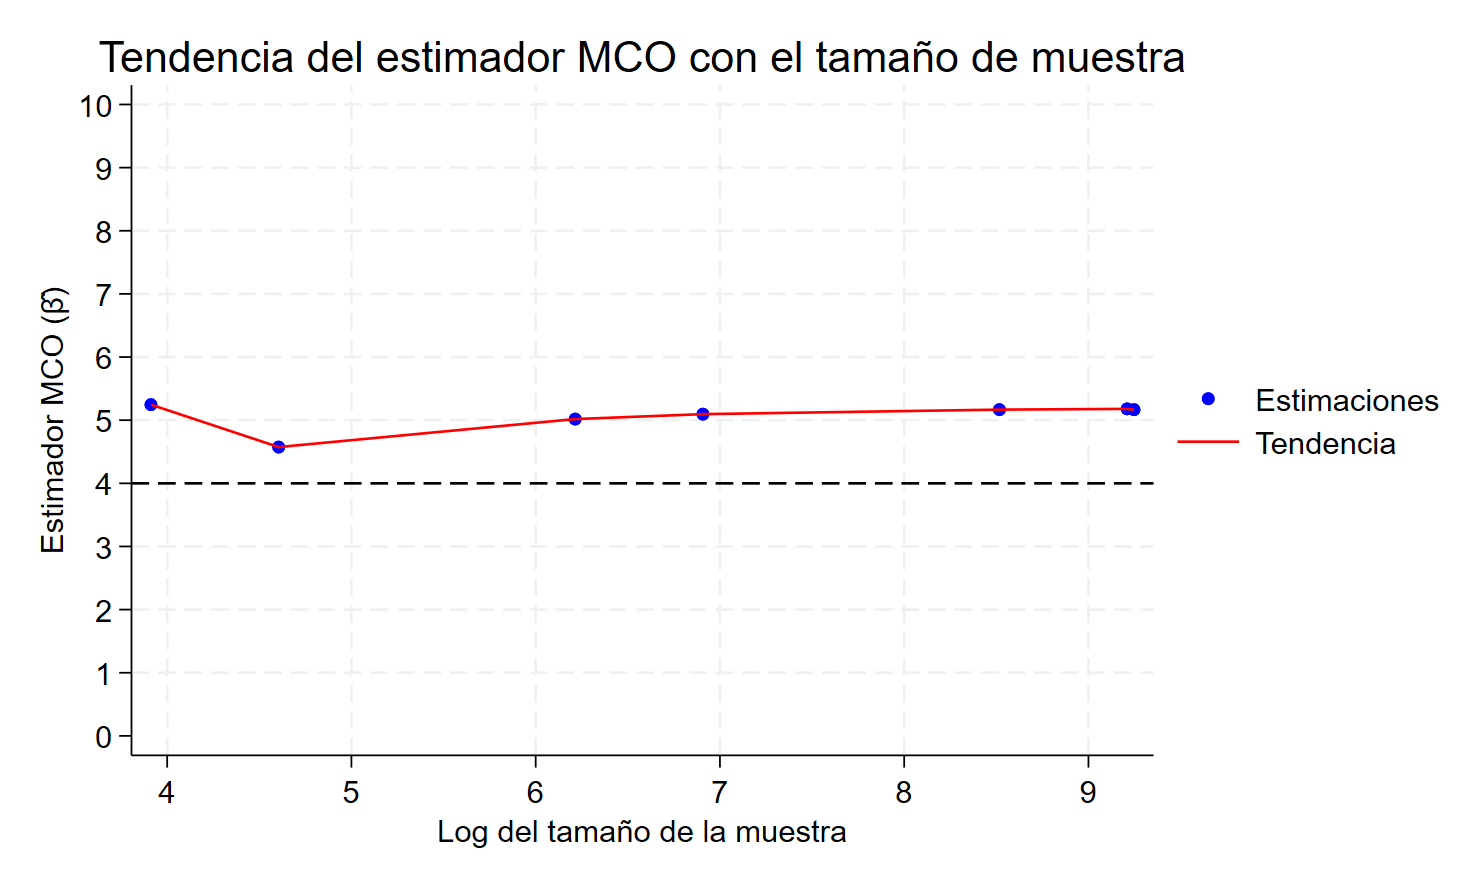
\includegraphics[width=0.8\textwidth]{output/figures/graficoconinter.png} 
    %\caption{Descripción de la imagen.}
    \label{fig:mi_grafico}
\end{figure}Se estima la regresión para muestras de tamaño 50, 100, 500, 1000, 5000, 10000  y el total de la muestra que fueron 10380 datos. A continuación se detalla una tabla con los resultados del estimador por MCO (beta\_hat) para los logaritmos de las muestras (log\_n): 
\begin{table}[H]
    \centering
    \caption{Resultados de log\_n y beta\_hat}
    \begin{tabular}{cc}
        \toprule
         \textbf{log\_n} & \textbf{beta\_hat} \\
        \midrule
        3.912023  & 5.2463235 \\
         4.6051702 & 4.5747697 \\
         6.2146081 & 5.0180653 \\
         6.9077553 & 5.0959556 \\
        8.5171932 & 5.1672351 \\
         9.2103404 & 5.1790206 \\
        9.2477325 & 5.1669749 \\
        \bottomrule
    \end{tabular}
    \label{tab:resultados}
\end{table}
Estos resultados dan intuición sobre la presencia de un posible sesgo que esté sobreestimando el efecto de interés. Se puede observar que el estimador tiende a estabilizarse alrededor de un valor sobre 5, mientras que el valor teórico esperado es 4. 

        \end{solucion}

    \item[8.] Demuestre que, asintóticamente, el estimador MCO sobrestima el efecto $\tau$. Es decir, pruebe que  
\[
\plim_{n \to \infty} \hat{\tau}_{MCO} > \tau.
\]

    Usando su demostración y la base de datos que tiene, de una estimación del valor de $\theta$. ¿Este estimador es coherente con los resultados que ha estado obteniendo?
     \begin{solucion}
       
        \begin{proof}
       Considere la regresión $Y_i =\alpha+ \tau^* D_i + u_i$. Sabemos 
\begin{align*}
    \hat{\tau}^*_{MCO} &=(X'X)^{-1} X' y \\
    &= (X'X)^{-1} X' (X \tau^* + \epsilon) \\
    &= (X'X)^{-1} X' (X (\tau + \theta) + \epsilon) \\
    &= (X'X)^{-1} X' X \tau + (X'X)^{-1} X' X\theta + (X'X)^{-1} X' \epsilon \\
    &= \tau + \theta + (X'X)^{-1} X' \epsilon \\
    &= \tau + \theta + \left( \frac{X'X}{N} \right)^{-1} \left( \frac{X'\epsilon}{N} \right) \quad \text{(multiplicando y dividiendo por N)} \\
    &= \tau + \theta + \left( \frac{1}{N} \sum_{i=1}^{N} x_i x_i' \right)^{-1} \left( \frac{1}{N} \sum_{i=1}^{N} x_i \epsilon_i \right).
  \end{align*}
  Ahora, aplicando el p-lim tenemos:
  \begin{align*}
    \text{plim } \hat{\tau}^*_{MCO} &= \text{plim} \left( \tau + \theta+ \left( \frac{1}{N} \sum_{i=1}^{N} x_i x_i' \right)^{-1} 
    \left( \frac{1}{N} \sum_{i=1}^{N} x_i \epsilon_i \right) \right) \\
    &= \text{plim } \tau + \text{plim } \theta +\text{plim} \left( \left( \frac{1}{N} \sum_{i=1}^{N} x_i x_i' \right)^{-1} 
    \left( \frac{1}{N} \sum_{i=1}^{N} x_i \epsilon_i \right) \right) \\
    &= \tau +\theta+ \text{plim} \left( \frac{1}{N} \sum_{i=1}^{N} x_i x_i' \right)^{-1} 
    \cdot \text{plim} \left( \frac{1}{N} \sum_{i=1}^{N} x_i \epsilon_i \right) \\
      &= \tau +\theta + \text{plim} E[x_i x_i'] ^{-1} \text{plim} E[x_i \epsilon_i] \qquad \text{(por ley débil de grandes números) }\\
      &= \tau +\theta + \text{plim} E[x_i x_i'] ^{-1} 0 \qquad \text{(usando exogeneidad débil) }\\
       &= \tau +\theta
    \end{align*}
   Como $\theta > 0$ entonces se tiene que $\text{plim } \hat{\tau}^*_{MCO}=\tau + \theta >\tau$.
        \end{proof}
        Ahora, como empíricamente obtuvimos $\hat{\tau}^*_{MCO} \approx 5.16$ y teóricamente $\tau \approx 4$ entonces el tenemos un sesgo, ahora bien este podría ser incluso mayor a $\approx 1.16$, pues hay una variable omitida importante, que es hacer colaborado o no.  Esto es congruente con los resultados obtenidos en cuanto el estimador empírico es mayor que el estimador teórico.\textcolor{red}{incluir valor del sesgo}
        \end{solucion}

    \item[9.] Proponga una metodología para recuperar estimadores consistentes de $\tau$ y de $\theta$. 

    \begin{itemize}
        \item[a.] Escriba detalladamente la especificación que va a estimar.
        

        \item[b.] Justifique por qué su propuesta será exitosa.

        \item[c.] Estime la regresión $Y_i = \alpha + \tau D_i + u_i$.

        \item[d.] Estime la especificación que usted propuso en el inciso a.

        \item[e.] Reporte los resultados de los incisos c., y d.en una tabla, compárelos y concluya. 

    \end{itemize}
     \begin{solucion}
        
        a.)Sea C una variable dummy tal que:
        \[
C_i =
\begin{cases} 
1, & \text{si el proyecto del investigador } i \text{ es colaborativo} \\
0, & \text{de lo contrario}
\end{cases}
\]
Se propone estimar la regresión: 
\begin{gather}\label{sinsesgoautores}
    Y_i = \alpha+\tau D_i + \theta C_i D_i+ e_i
\end{gather}


       


        b.) Esta propuesta será exitosa porque permite aislar el efecto de solamente publicar en un trending research topic, cuando el proyecto no es colaborativo. \textcolor{red}{revisar}. \\
          
        
        Note que para los investigadores que escriben en trending research topics y que colaboran tendremos que:
       \[
\mathbb{E}[Y \mid D=1, C=1] = \alpha + \tau + \theta +\mathbb{E}[e \mid D, C]
\]
Mientras que si escriben en trending research topics pero no colaboran tendremos que:
       \[
\mathbb{E}[Y \mid D=1, C=0] = \alpha + \tau +\mathbb{E}[e \mid D, C]  
\]
Finalmente, si no escriben en trending reserach topic (ergo no colaboran en trending reserach topic, pues solo es posible colaborar cuando se trabaja en un trending research topic) tenemos:
  \[
\mathbb{E}[Y \mid D=0, C=0] = \alpha +\mathbb{E}[e \mid D, C]  
\]
Luego, suponiendo que hay una correcta aleatorización entre el grupo de tratados y el grupo de control, tendremos que:
\begin{itemize}
    \item El efecto de solamente publicar en un trending research topic versus no publicar, sobre el número de citas que recibe un investigador está dado por:
    \[
\mathbb{E}[Y \mid D=1, C=0]- \mathbb{E}[Y \mid D=0, C=0] =  \tau   
\]

    \item El efecto de publicar en un trending research topic versus no publicar, y además colaborar, sobre el número de citas que recibe un investigador está dado por:
    \[
\mathbb{E}[Y \mid D=1, C=1]- \mathbb{E}[Y \mid D=0, C=0] = \tau +\theta
\]


\end{itemize}

c.)\begin{table}[H]
    \centering
    \caption{Efecto de \textit{trending\_topic} sobre \textit{author\_citations}}
    \label{tab:resultados}
    \begin{tabular}{l c}
        \toprule
        & Número total de citaciones\\
        \midrule
        \textbf{Trending Topic} & 5.167*** \\
        & (0.051) \\
        \textbf{Constante} & 12.120*** \\
        & (0.023) \\
        \midrule
        Observaciones & 10,381 \\
        Controles & No \\
        R cuadrado ajustado & 0.4958 \\
        \bottomrule
    \end{tabular}
    
    \vspace{0.3cm}
    \footnotesize{*** p$<$0.01, ** p$<$0.05, * p$<$0.1. \\
    Errores estándar robustos a heterocedasticidad entre paréntesis.}
\end{table}

El coeficiente estimado de $\tau$ es 5.167. Indica que en promedio, los investigadores que publican en trending research topic reciben 5.167 más citas que los que no lo hacen. Este valor es  mayor que el valor teórico esperado de 4, lo cual indica que el sesgo es positivo y que tiene una magnitud de $\approx 1.167$.

        d.)
        \begin{table}[H]
    \centering
    \caption{Efecto de \textit{trending\_topic} y su interacción con \textit{collaborative} sobre \textit{author\_citations}}
    \label{tab:resultados}
    \begin{tabular}{l c}
        \toprule
        & Número total de citaciones \\
        \midrule
        \textbf{Trending Topic} & 3.895*** \\
        & (0.066) \\
        \textbf{Trending Topic $\times$ Collaborative} & 2.552*** \\
        & (0.088) \\
        \textbf{Constante} & 12.120*** \\
        & (0.022) \\
        \midrule
        Observaciones & 10,381 \\
        R-cuadrado ajustado & 0.5338 \\
        Root MSE & 2.0232 \\
        \bottomrule
    \end{tabular}
    
    \vspace{0.3cm}
    \footnotesize{*** p$<$0.01, ** p$<$0.05, * p$<$0.1. \\
    Errores estándar en paréntesis.}
\end{table}
Note que el sesgo por variable omitida no era simplemente restar el valor teórico del empírico obtenido inicialmente, sino que es más complejo porque también afecta los errores residuales.
\textcolor{red}{pero el sesgo no deberia ser como 1.5 algo horario?}
        
        \end{solucion}
    

\end{itemize}
\bigskip



%%%%%%%%%% Punto 2 %%%%%%%%%%%%%
\section*{Segundo Ejercicio}
El teorema de Frisch-Waugh-Lovell es uno de los resultados más importantes en econometría, pues permite entrever los mecanismos detrás de la estimación de los modelos de regresión lineal cuando se incluyen varias variables independientes. En este punto vamos a estudiar las implicaciones de este teorema.


\begin{enumerate}
    \item Considere el modelo de regresión múltiple en notación matricial con \(n\) observaciones, una variable dependiente y \(k\) variables independientes:
    
    \begin{align}\label{EQ:modelInicial}
        \mathbf{y} &= \mathbf{X}\beta + \boldsymbol\epsilon
    \end{align}

    Considere las siguientes definiciones: \\ 
    
    \begin{mdframed}
        \textbf{Def.\ (Proyección ortogonal):} Se dice que una matriz cuadrada \( \mathbf{P} \) de valores reales es una matriz de proyección ortogonal si cumple las siguientes propiedades:
        \begin{enumerate}
            \item \( \mathbf{P}^2 = \mathbf{P} \) (idempotencia).
            \item \( \mathbf{P}' = \mathbf{P} \) (simetría).
        \end{enumerate}
     \end{mdframed}
    \vspace{1em}
    
    \begin{mdframed}
    \textbf{Def.\ (Matriz de aniquilación):} Sea \( \mathbf{X} \) una matriz de tamaño \( n \times k \) de rango completo. La matriz de aniquilación asociada a \( \mathbf{X} \) es una matriz \( \mathbf{M} \) definida como:
    \[
    \mathbf{M} = \mathbf{I}_n - \mathbf{P},
    \]
    donde \( \mathbf{I}_n \) es la matriz identidad de tamaño \( n \times n \) y \( \mathbf{P} \) es la matriz de proyección ortogonal sobre el espacio columna de \( \mathbf{X} \).
    \end{mdframed}
    \vspace{1em}
    
    De forma intuitiva, una \textbf{matriz de proyección ortogonal} es una herramienta que nos permite ``proyectar'' un vector sobre un subespacio, de modo que el resultado es el punto del subespacio más cercano al vector original. El término ``ortogonal'' significa que la diferencia entre el vector original y su proyección (es decir, el ``residuo'' de la proyección) es perpendicular al subespacio. Esto se traduce en que la proyección minimiza la distancia entre el vector original y el subespacio.
    
    \bigskip Por otro lado, la \textbf{matriz de aniquilación} elimina la parte del vector que la matriz de proyección habría capturado. Lo que queda es la porción del vector que no se puede representar en ese subespacio, es decir, el ``residuo'' que no encaja en el subespacio. \\
    
    \begin{enumerate}
        \item Demuestre que \(\mathbf{P} \equiv \mathbf{X}(\mathbf{X'}\mathbf{X})^{-1}\mathbf{X'}\) es una matriz de proyección ortogonal.
        \item Sea \(\mathbf{\hat{y}} = \mathbf{X}\hat\beta\) el vector de valores predichos de \(\mathbf{y}\), donde \(\hat\beta\) es el estimador de MCO de \(\beta\). Demuestre que \(\mathbf{\hat{y}} = \mathbf{P}\mathbf{y}\).
        \item Sea \(\hat{\epsilon} = \mathbf{y} - \mathbf{\hat{y}}\) el vector de residuales de la regresión. Demuestre que \(\hat{\epsilon} = \mathbf{M} \mathbf{y}\).
    \end{enumerate}
    \bigskip

    \item Considere el modelo \eqref{EQ:modelInicial} bajo la siguiente partición de $\mathbf{X}$\footnote{Una partición de una matriz se denota con el uso de corchetes cuadrados $\mathbf{X} = [\mathbf{X}_1 \, \mathbf{X}_2]$. Note que esto no es un producto de matrices, sino simplemente una forma de decir que hay dos grupos de interés distintos.}:

    \begin{align}
    \begin{split}
        \textbf{y} &= \textbf{X}_1 \beta_1 + \textbf{X}_2 \beta_2 + \boldsymbol\epsilon, \label{EQ:modelParticionado} \\
    \end{split}
    \end{align}

    donde $\textbf{X}_1$ y $\textbf{X}_2$ son matrices y $\beta_1$ y $\beta_2$ son vectores. Suponga que el grupo 1 de variables tiene $k_1$ variables explicativas y que el grupo 2 tiene $k_2$ variables, donde $k_1 + k_2 = k$.

    Partiendo de las condiciones de primer orden del estimador de mínimos cuadrados ordinarios (MCO), demuestre que:

    \begin{align}
        \begin{bmatrix}
            \textbf{X}_{1}' \\
            \textbf{X}_{2}'
        \end{bmatrix} 
            [ \textbf{X}_1  \hspace{0.2em}  \textbf{X}_2 ]
        \begin{bmatrix}
            \hat\beta_1 \\
            \hat\beta_2
        \end{bmatrix} &= 
        \begin{bmatrix}
            \textbf{X}_{1}' \\
            \textbf{X}_{2}'
        \end{bmatrix}
        \textbf{y},\label{EQ:particionado}
    \end{align}

     y realice la expansión correspondiente para obtener un sistema lineal de dos ecuaciones: 

    \begin{equation}
    \begin{cases}
    \textbf{X}_{1}'\textbf{X}_{1}\hat{\beta}_1 + \textbf{X}_{1}'\textbf{X}_{2}\hat{\beta}_2 = \textbf{X}_{1}'\textbf{y} & \text{(3.1)} \\
    \textbf{X}_{2}'\textbf{X}_{1}\hat{\beta}_1 + \textbf{X}_{2}'\textbf{X}_{2}\hat{\beta}_2 = \textbf{X}_{2}'\textbf{y} & \text{(3.2)}
    \end{cases}
    \end{equation}

    \bigskip

\begin{solucion}

\begin{lemma}\label{lma1}
La transpuesta de la matríz particionada  \( X = [X_1, X_2] \) es
\[
X^\top = 
\begin{bmatrix}
X_1^\top \\
X_2^\top
\end{bmatrix}
\]
   
\end{lemma}

Primero veamos cómo llegar a  \ref{EQ:particionado} partiendo de \ref{EQ:modelParticionado}

\begin{proof}  

Nota: En la demostración omitiremos el uso de símbolos en negrilla para simplificar la notación.\\

Si escribimos el vector de residuales como:
\begin{equation}
\hat{\epsilon} = y - X\hat{\beta} \label{eq:residuales}
\end{equation}

y, antes de reemplazar la matriz $X$ y el vector $\hat{\beta}$ por sus respectivas versiones particionadas, recordemos que las condiciones de primer orden del estimador de MCO partiendo de \ref{eq:residuales} son:

\begin{align}
\frac{\partial \hat{\epsilon}'\hat{\epsilon}}{\partial \hat{\beta} } &= -2X'y + 2X'X\hat{\beta} = 0 \notag \qquad (\text{factorizando el 2}) \\
% Factorizando el 2
X'X\hat{\beta} - X'y &= 0 \notag \qquad (\text{restando $X'y$ a ambos lados})  \\
X'X\hat{\beta} &= X'y \label{eq:condiciones} 
\end{align}

Ahora, reemplazamos $X$ y $\hat{\beta}$ por sus versiones particionadas, y teniendo cuidado de que la dimensión $k$ respete $k_1 + k_2 = k$, y siguiendo el Lema \ref{lma1}:

\begin{align}
\begin{bmatrix}
X_1' \\
X_2'
\end{bmatrix}
\begin{bmatrix}
X_1 & X_2
\end{bmatrix}
\begin{bmatrix}
\hat{\beta}_1 \\
\hat{\beta}_2
\end{bmatrix} &=
\begin{bmatrix}
X_1' \\
X_2'
\end{bmatrix}
y
\end{align}

y llegamos a la expresión deseada. $\square$
\end{proof}


\textbf{Expanding the previous expression}

\[
\begin{bmatrix}
X_1^\top X_1 & X_1^\top X_2 \\
X_2^\top X_1 & X_2^\top X_2
\end{bmatrix}
\begin{bmatrix}
\hat{\beta}_1 \\
\hat{\beta}_2
\end{bmatrix}
=
\begin{bmatrix}
X_1^\top \\
X_2^\top
\end{bmatrix} y.
\]

From which we derive the following system:

\[
X_1^\top X_1 \hat{\beta}_1 + X_1^\top X_2 \hat{\beta}_2 = X_1^\top y,
\]

\[
X_2^\top X_1 \hat{\beta}_1 + X_2^\top X_2 \hat{\beta}_2 = X_2^\top y.
\]

\(\square\)

\end{solucion}


%██████  ██████  
%██   ██      ██ 
%██████   █████  
%██   ██      ██ 
%██████  ██████  
                
            
    \item Demuestre que la matriz $\textbf{P}_1 \equiv \textbf{X}_1(\textbf{X}_1'\textbf{X}_1)^{-1}\textbf{X}_1'$ es una matriz de proyección ortogonal y defina la matriz de aniquilación $\textbf{M}_1$ asociada a $\textbf{X}_1$. Demuestre que $\textbf{M}_1$ también es una matriz de proyección ortogonal. Así mismo, demuestre que 

    \begin{enumerate}\label{aniquiladoranotaciona}
        \item $M_1\textbf{X}_1 = \textbf{0}$ (es por esta razón que la matriz se denomina como aniquiladora).
        \item $M_1\boldsymbol\epsilon = \boldsymbol\epsilon$.
    \end{enumerate}


\begin{solucion}

Veamos que $\boldsymbol{\hat{y}} = \boldsymbol{X}\boldsymbol{\hat{\beta}}$ es la proyección de $\boldsymbol{y}$ sobre el espacio generado por $\boldsymbol{X}$. Para ello, debemos demostrar que $\boldsymbol{y} - \boldsymbol{\hat{y}}$ es ortogonal a $\boldsymbol{X}$.

Ahora veamos que la matriz $P_1 = X_1(X_1'X_1)^{-1}X_1'$ es una proyección ortogonal. Para ello debemos ver si esta es idempotente y simétrica

\textbf{Idempotencia:}
\begin{proof}
\begin{align*}
    P_1^2 &= X_1(X_1'X_1)^{-1}X_1'X_1(X_1'X_1)^{-1}X_1' \\
    &= X_1(X_1'X_1)^{-1}X_1' \\
    &= P_1
\end{align*}
\end{proof}

\textbf{Simetría:}
\begin{proof}
\begin{align*}
    P_1' &= \left( X_1(X_1'X_1)^{-1}X_1' \right)' \\
    &= X_1 \left( (X_1'X_1)^{-1} \right)' X_1' \\
    &= X_1 \left( (X_1'X_1)' \right)^{-1} X_1' \\
    &= X_1 (X_1'X_1)^{-1} X_1' \\
    &= P_1
\end{align*}
\end{proof}

Por otro lado, veamos que la matriz de aniquilación $M_1 = I - P_1$ es una proyección ortogonal. Para ello debemos ver si esta es idempotente y simétrica.

\textbf{Idempotencia:}
\begin{proof}
\begin{align*}
    M_1^2 &= (I - P_1)(I - P_1) \\
    &= I - P_1 - P_1 + P_1^2 \\
    &= I - P_1 - P_1 + P_1 \\
    &= I - P_1 \\
    &= M_1
\end{align*}
\end{proof}

\textbf{Simetría:}
\begin{proof}
\begin{align*}
    M_1' &= (I - P_1)' \\
    &= I' - P_1' \\
    &= I - P_1 \\
    &= M_1
\end{align*}
\end{proof}

\bigskip

% ██████  ██████      █████  
% ██   ██      ██    ██   ██ 
% ██████   █████     ███████ 
% ██   ██      ██    ██   ██ 
% ██████  ██████  ██ ██   ██ 
                           
Ahora veamos que $M_1$ aniquila a $X_1$. Para ello, debemos demostrar que $M_1X_1 = \boldsymbol{0}$.
\begin{proof}
\begin{align*}
    M_1X_1 &= (I - P_1)X_1 \\
    &= X_1 - P_1X_1 \\
    &= X_1 - X_1(X_1'X_1)^{-1}X_1'X_1 \\
    &= X_1 - X_1 \\
    &= \boldsymbol{0}
\end{align*}
\end{proof}



% ██████  ██████     ██████  
% ██   ██      ██    ██   ██ 
% ██████   █████     ██████  
% ██   ██      ██    ██   ██ 
% ██████  ██████  ██ ██████  
                           
Por otro lado, veamos que $M_1\epsilon = \epsilon$. Esta propiedad nos dice que la matriz de aniquilación $M_1$ no afecta a $\epsilon$.
Para ello, debemos demostrar que $M_1\epsilon = \epsilon$.

\begin{proof}
    \begin{align}
        M_1\epsilon &= (I - P_1)\epsilon \\
        &= \epsilon - P_1\epsilon \qquad (\text{por exogeneidad débil}) \\
        &= \epsilon 
    \end{align}
\end{proof}

\textbf{NOTA:}
Tenemos por supuesto del modelo de regresión lineal que las variables independientes no tienen información para predecir $\epsilon$, lo que llamamos \textbf{exogeneidad estricta}, que implica exogeneidad débil.

\end{solucion}

    \item Sean:
    
    \begin{itemize}\label{aniquiladoranotacion}
        \item $\boldsymbol{\Tilde{X}_2} =  M_1\textbf{X}_2$.
        \item $\boldsymbol{\Tilde{y}} =  M_1\textbf{y}$.
    \end{itemize}

    Interprete brevemente $\boldsymbol{\Tilde{X}_2}$ y $\boldsymbol{\Tilde{y}}$ en sus propias palabras y luego demuestre que

    \begin{equation}\label{eq:equiv}
        \textbf{y} = \textbf{X}_1\beta_1 + \textbf{X}_2\beta_2 + \boldsymbol\epsilon \quad \textrm{puede re-escribirse como} \quad \boldsymbol{\Tilde{y}} =\boldsymbol{\Tilde{X}_2}\beta_2 + \boldsymbol\epsilon
    \end{equation}

    \bigskip Después, usando las ecuaciones (3.1) y (3.2), demuestre que:
    
    \begin{equation}\label{eq:resid}
        \hat\beta_2 = (\boldsymbol{\Tilde{X}_2'}\boldsymbol{\Tilde{X}_2})^{-1}\boldsymbol{\Tilde{X}_2'}\boldsymbol{\Tilde{y}}.
    \end{equation}

    \textbf{Pista:} Multiplique a ambos lados de la ecuación (3.1) por $\textbf{X}_1(\textbf{X}_1'\textbf{X}_1)^{-1}$ y obtenga una ecuación para $\textbf{X}_1\hat\beta_1$ en función de la matriz de proyección $\textbf{P}_1$ y reemplace en (3.2). Asuma que la matriz $\boldsymbol{\Tilde{X}_2}$ es de rango completo. 

\begin{solucion}
\textbf{Paso 1: Interpretación}

\begin{itemize}
    \item $P_1$ proyecta cualquier vector sobre el espacio generado por $\mathbf{X_1}$. El hecho de que le llamen a la matriz de proyección ortogonal "matriz sombrero" o \textit{hat matrix} es precisamente porque lleva a los valores predichos. Usando la matriz completa (no la particionada) sabemos que $\hat{\mathbf{y}}=\mathbf{Py}$, porque además de "ponerle el sombrero" a las $y$'s también extrae la parte que es explicada por los Xs. En el contexto de la $P_1$ esta extrae la parte del vector explicada por $\mathbf{X}_1$.
    \item Dado que $P_1$ extrae de un vector el componente del espacio columna de $\mathbf{X}_1$,  entonces $M_1$ elimina o "aniquila" el componente de $X_1$, dejándo solo aquello que es ortogonal a $\mathbf{X}_1$, precisamente la razón por la cual $M_1\mathbf{X}_1=0$. 
\end{itemize}

\textbf{Paso 2: Transformación del Modelo de Regresión}

El modelo de regresión original es:

$$
\mathbf{y} = \mathbf{X}_1 \boldsymbol{\beta}_1 + \mathbf{X}_2 \boldsymbol{\beta}_2 + \boldsymbol{\epsilon}.
$$

Premultiplicando por $M_1$ en ambos lados:

$$
M_1 \mathbf{y} = M_1 (\mathbf{X}_1 \boldsymbol{\beta}_1 + \mathbf{X}_2 \boldsymbol{\beta}_2 + \boldsymbol{\epsilon}).
$$

Dado que $M_1$ es una matriz aniquiladora que proyecta fuera del espacio columna de \( \mathbf{X}_1 \), se cumple que:

\[
M_1 \mathbf{X}_1 = 0.
\]

Además, sabemos del ejercicio anterior que $M_1\boldsymbol{\epsilon}=\boldsymbol{\epsilon}$. Por lo tanto, el término \( M_1 \mathbf{X}_1 \boldsymbol{\beta}_1 \) desaparece, dejando:

\[
M_1 \mathbf{y} = M_1 \mathbf{X}_2 \boldsymbol{\beta}_2 +\boldsymbol{\epsilon}.
\]

Usando nuestras definiciones lleamos a lo deseado:

\[
\tilde{\mathbf{y}} = \tilde{\mathbf{X}}_2 \boldsymbol{\beta}_2 + \boldsymbol{\epsilon}.
\]


Esto muestra que el modelo transformado solo involucra las componentes de \( \mathbf{X}_2 \) y \( \mathbf{y} \) que son ortogonales a \( \mathbf{X}_1 \), reduciendo efectivamente la regresión a un problema equivalente en el complemento ortogonal de \( \mathbf{X}_1 \).


\textbf{Paso 3: Demostración OLS}


A continuación omitiremos el formato de negrilla pero de todas formas corresponde a las matrices $X=[X_1 X_2]$. Asimismo, $y\in \mathbb{R}^N$.

Tomamos (3.1) y premultiplicamos por $X_1 (X_1'X_1)^{-1}$:

\begin{align*} 
X_1 (X_1'X_1)^{-1} X_1'X_1 \hat{\beta}_1 + P_{1} X_2 \hat{\beta}_2 &= P_{1} \\
X_1 \hat{\beta}_1 &= P_{1} y - P_{1} X_2 \hat{\beta}_2 \quad (*)
\end{align*}

Tomamos \((*)\) y reemplazamos en (3.2):
\begin{align}
X_2' P_{1} y - X_2' P_{1} X_2 \hat{\beta}_2 + X_2' X_2 \hat{\beta}_2 &= X_2'y \notag \\
- X_2' P_{1} X_2 \hat{\beta}_2 + X_2' X_2 \hat{\beta}_2 &= X_2'y - X_2' P_{1} y \label{eq:ej4.1}\\
\end{align}

Para el lado derecho (RHS) de \ref{eq:ej4.1} usamos el hecho de que $M_1$ es idempotente y simétrica, y las definiciones de $\tilde{y}$ y $\tilde{X_2}$:

\begin{align}
&= X_2'(y-P_1y) \notag \\
&= X_2'M_1y \qquad \text{(por propiedades de $M_1$ )} \notag \\
&= X_2'M_1 M_1 y \qquad \text{Como $\tilde{X_2'}= (M_1X_2)' = X_2'M_1$} \notag \\
&= \tilde{X_2'}\tilde{y} \label{eq:ej4.RHS}
\end{align}

Para el lado izquierdo (LHS) de \ref{eq:ej4.1}:


\begin{align}
- X_2' P_{1} X_2 \hat{\beta}_2 + X_2' X_2 \hat{\beta}_2 &= \notag  \\
X_2' X_2 \hat{\beta}_2 - X_2' P_{1} X_2 \hat{\beta}_2  &=  \notag \\
(X_2' X_2 - X_2' P_{1} X_2 ) \hat{\beta}_2  &=  \notag \\
(X_2'(\mathbb{I}_N - P_1) X_2 ) \hat{\beta}_2  &=  \notag \\
 (X_2'M_1X_2)\hat{\beta}_2&= \notag \qquad \text{por propiedades de $M_1$} \\
 (X_2'M_1M_1X_2)\hat{\beta}_2&= \notag \\
  (\tilde{X_2'}\tilde{X_2})\hat{\beta}_2&= \label{eq:ej4.LHS}
\end{align}

Ahora, de \ref{eq:ej4.LHS} y \ref{eq:ej4.RHS}, premultiplicamos a ambos lados por la inversa de $\tilde{X'}_2\tilde{X_2}$, que podemos obtener por supuesto de que tiene rango completo:

\begin{align*}
    (\tilde{X_2'}\tilde{X_2})\hat{\beta}_1 &= \tilde{X_2'}\tilde{y} \\
\hat{\beta}_1 &= (\tilde{X_2'}\tilde{X_2})^{-1} \tilde{X_2'}\tilde{y}
\end{align*}

y obtuvimos lo que queríamos.
\end{solucion}
    

    \bigskip

    \item Finalmente, en este último inciso va a mostrar que los estimadores que obtuvo anteriormente son los mismos que los que obtendría realizando MCO sobre la segunda regresión de~\eqref{eq:equiv}. Partiendo de la ecuación~\eqref{eq:resid} y usando las definiciones de  $\boldsymbol{\Tilde{X}_2}$ y de  $\boldsymbol{\Tilde{y}}$, demuestre que

    \begin{equation}
        \hat\beta_2 = (\boldsymbol{\Tilde{X}_2'}\boldsymbol{\Tilde{X}_2})^{-1}\boldsymbol{\Tilde{X}_2'}\textbf{y}.
    \end{equation}

    Note que $\boldsymbol{\Tilde{y}} \neq \textbf{y}$, pues la primera es afectada por la matriz de aniquilación $M_1$ y la segunda es el vector de la variable independiente sin ninguna alteración. ¿Cuál es la diferencia entre el resultado que obtuvo en el inciso 4. vs el de este inciso?

\begin{solucion}

\textbf{Demostración}
Usando nuestras definiciones tenemos que 
\begin{align*}
\tilde{X}'_2&=(M_1X_2)' \\
&= X_2'M_1' \\
&= X_2' M_1 \qquad \text{Por la simetría de $M_1$ }.
\end{align*}


Procedemos: 

\begin{align*}
\hat{\beta}_2 
 &= (\tilde{X}_2^\prime \tilde{X}_2)^{-1} \tilde{X}_2^\prime \tilde{y}\\
 &= (\tilde{X}_2^\prime \tilde{X}_2)^{-1} X_2^\prime M_1 M_1\,y \text{ (Usando que $M_1\,y=\tilde{y}$, $M_1\,X_2=\tilde{X}_2$)}\\
 &= (\tilde{X}_2^\prime \tilde{X}_2)^{-1} X_2^\prime M_1\,y
 \quad (\text{por }M_1^2 = M_1)\\
 &= (\tilde{X}_2^\prime \tilde{X}_2)^{-1} \tilde{X}_2^\prime \,y
\quad (\text{pues }  \tilde{X}_2^\prime = X_2^\prime M_1)
\end{align*}


\textbf{Interpretación Diferencia}
Al usar \( \tilde{y} \), se elimina cualquier influencia de \( X_1 \) en la variable dependiente \( y \). Lo que se obtiene es la estimación de \( \beta_2 \) después de haber controlado por \( X_1 \) tanto en el lado de las variables dependientes como en el lado de las independientes. En el segundo término, se usa el vector \( y \) original, sin residualizar. En este caso, el vector \( y \) no se ajusta explícitamente por \( X_1 \), pero el hecho de que \( \tilde{X}_2 \) ya sea residualizado (es decir, ya se haya controlado \( X_1 \) en el lado de las variables independientes) controla indirectamente el efecto de \( X_1 \) en \( y \).

En términos de covarianzas, la estimación de \( \beta_2 \) se puede expresar de la siguiente forma:

\[
\hat{\beta}_2 = \frac{\text{cov}(\tilde{y}, \tilde{X}_2)}{\text{var}(\tilde{X}_2)} \quad \text{y} \quad \hat{\beta}_2 = \frac{\text{cov}(y, \tilde{X}_2)}{\text{var}(\tilde{X}_2)}.
\]

Los numeradores de ambas expresiones son equivalente por el hecho de que \( \tilde{X}_2 \) no tiene niguna influencia de \( X_2 \) entonces no importa si no se descuenta la influencia de \( X_1 \) sobre \( y \) en el resultado de este inciso, porque \( X_1 \) no va a ejercer ninguna influencia sobre la relación entre 
$\text{cov}(y, \tilde{X}_2)$

\colorbox{yellow}{HELP!!!}

\end{solucion}

    \item El estimador de Mínimos Cuadrados Ordinarios (MCO) es ampliamente conocido, estudiado y utilizado en econometría. Un resultado fundamental en esta disciplina es el Teorema de Gauss-Markov, el cual establece que, bajo los supuestos del Modelo Clásico Lineal, el estimador por MCO es BLUE (Best Linear Unbiased Estimator). Es decir, dentro de la familia de estimadores lineales insesgados, MCO es el que tiene menor varianza.\footnote{Hansen (2022) va más allá al demostrar que OLS también es \textit{BUE} (\textit{Best Unbiased Estimator}), un resultado aún más fuerte aunque, quizá, menos conocido (y con peor nombre) que la denominación ``BLUE''.}  
    
    En este último inciso ústed buscará demostrar el vínculo entre el teorema Frisch-Waugh-Lovell y Gauss-Markov. Considere el modelo de regresión lineal
\begin{equation}\label{EQ:modeloGM}
    \mathbf{y} = \mathbf{X}\beta + \boldsymbol\epsilon,
\end{equation}
donde \(\mathbb{E}[\boldsymbol\epsilon] = \mathbf{0}\) y \(\mathrm{Var}(\boldsymbol\epsilon)=\sigma^2 \mathbf{I}_n\). Recordemos que el estimador de mínimos cuadrados (MCO) se puede escribir como
\[
\hat{\beta} = (\mathbf{X}'\mathbf{X})^{-1}\mathbf{X}'\mathbf{y},
\]
y que su interpretación geométrica es la proyección ortogonal de \(\mathbf{y}\) sobre el espacio columna de \(\mathbf{X}\); es decir, \(\hat{\mathbf{y}} = \mathbf{P}\mathbf{y}\) con
\[
\mathbf{P} = \mathbf{X}(\mathbf{X}'\mathbf{X})^{-1}\mathbf{X}'.
\]

\begin{mdframed}
\textbf{Teorema \textit{Gauss-Markov}}
Bajo los supuestos del modelo clásico lineal, \(\hat{\beta}\) es el \emph{Best Linear Unbiased Estimator} (BLUE), es decir
\begin{align}
   \text{Var}(\hat{\beta}) \geq \sigma^2 (\mathbf{X}' \mathbf{X})^{-1}    \tag{Gauss-Markov}
\end{align}
\end{mdframed}

\begin{itemize}
    \item[a)] Utilizando el Teorema de Frisch-Waugh-Lovell, demuestre que la estimación de \(\beta\) mediante la proyección ortogonal (es decir, mediante \(\hat{\beta} = (\mathbf{X}'\mathbf{X})^{-1}\mathbf{X}'\mathbf{y}\)) garantiza que toda variación en \(\mathbf{y}\) que no esté contenida en el espacio de \(\mathbf{X}\) es eliminada. En otras palabras, demuestre que los residuos
\[
\hat{\boldsymbol\epsilon} = \mathbf{y} - \mathbf{P}\mathbf{y} = (\mathbf{I}_n - \mathbf{P})\mathbf{y}
\]
son ortogonales a todo vector en dicho espacio.

 \begin{solucion}
  \begin{proof}
     Sea el vector \(\vec{v}  \in Span \{\ \vec{X_1}, \vec{X_2},.., \vec{X_k} \}\). Es decir $\vec{v}$ es un vector en el espacio generado por \( \vec{X_1}, \vec{X_2},.., \vec{X_k} \). Queremos mostrar que \( v \) es ortogonal a los residuos \( \hat{\epsilon} \). Es decir, que \( v^\top \hat{\epsilon} = 0 \).

Sabemos que \( X \) es una matriz de tamaño \( n \times k \), cuya \( i \)-ésima fila está dada por \( x_i = (x_{i1}, x_{i2}, \dots, x_{ik}) \).
Dado que \( v \) está en el espacio generado por las columnas de la matriz \( X = [\vec{X_1}, \vec{X_2},.., \vec{X_k}] \), entonces existe un vector de reales \( c = (c_1, c_2, \dots, c_k)^\top \) tal que:

\[
v = X c
\]

Entonces:
\begin{align*}
    v^\top \hat{\epsilon} & = (X c)^\top \hat{\epsilon}\\
    & = (Xc)^\top (I_n - P) y \quad \text{(Usando que $\hat{\epsilon}=My=(I_n - P)y$ )} \\
     & = c^\top X^\top y - c^\top X^\top P y \\
                       &= c^\top X^\top y - c^\top X^\top y \quad \text{(Usando que $X^\top P=(P X)^\top=X^\top$ )}\\
                       &= 0
\end{align*}

\end{proof}
La clave en esta prueba es que $X^\top P=X^\top$. Esto es porque  \( P = X (X^\top X)^{-1} X^\top \), y la propiedad de la proyección ortogonal implica que proyectar \( X \) sobre el espacio generado por sus columnas no cambia las columnas de \( X \).  La estimación de \( \beta \) mediante la proyección ortogonal \( \hat{\beta} = (X'X)^{-1} X'y \) garantiza que toda la variación de \( y \) que no está contenida en el espacio columna de \( X \) se elimina. Los residuos \( \hat{\epsilon} = (I_n - P)y \) son ortogonales a todo vector en dicho espacio.\textcolor{red}{revisar}

 \end{solucion}


    \item[b)] Sea \(\tilde{\beta} = \mathbf{A}\mathbf{y}\) un estimador lineal arbitrario de \(\beta\) (con \(\mathbf{A}\) una matriz no necesariamente igual a \((\mathbf{X}'\mathbf{X})^{-1}\mathbf{X}'\)). Demuestre que si \(\tilde{\beta}\) no se obtiene mediante la proyección ortogonal (es decir, si \(\mathbf{A}\) no ``elimina'' la variación irrelevante contenida en \(\mathbf{y}\)), entonces su varianza es mayor que la de \(\hat{\beta}\); esto es,
\[
\mathrm{Var}(\tilde{\beta}) \geq \sigma^2 (\mathbf{X}'\mathbf{X})^{-1}.
\]

\textit{Pistas:} A partir de la expresión de $\tilde{\beta}$ llegue a la condición \(\mathbf{A}\mathbf{X} = \mathbf{I}_k\), que a su vez implica que
\[
\mathbf{A} = (\mathbf{X}'\mathbf{X})^{-1}\mathbf{X}' + \mathbf{C}, \quad \text{con } \mathbf{C}\mathbf{X} = \mathbf{0}.
\]
Luego, exprese \(\tilde{\beta} = \hat{\beta} + \mathbf{C}\mathbf{y}\) y demuestre que
\[
\mathrm{Var}(\tilde{\beta}) = \sigma^2 (\mathbf{X}'\mathbf{X})^{-1} + \sigma^2\,\mathbf{C}\mathbf{C}'.
\] 

¿Qué puede concluir a partir de sus resultados?

\end{itemize}
    \end{enumerate}

    \bigskip


\Large\textbf{Parte práctica: Exposición a la violencia en Darfur}

\normalsize\bigskip En la región occidental de Darfur, Sudán, una campaña extremadamente violenta por parte del gobierno contra civiles se desarrolló a partir de 2003. Este conflicto es considerado un genocidio y resultó en acusaciones de crímenes de guerra y crímenes contra la humanidad por parte de la Corte Penal Internacional. Los mecanismos principales de violencia incluyeron fuertes bombardeos aéreos por parte del gobierno y ataques de la milicia pro-gubernamental llamada Janjaweed en cada pueblo. Es importante notar que algunos pueblos fueron más afectados por ser opositores al gobierno, y las mujeres eran un blanco de agresión sexual por parte de los Janjaweed, lo que las hacía más vulnerables a ser agredidas (Cinelli \& Hazlett, 2020)\footnote{Cinelli, C., \& Hazlett, C. (2020). Making sense of sensitivity: Extending omitted variable bias. \textit{Journal of the Royal Statistical Society Series B: Statistical Methodology}, 82(1), 39-67.
}.

\bigskip En este ejercicio, usted estudiará algunos obstáculos para obtener el efecto causal de ser víctima de los ataques frente lograr una resolución pacífica del conflicto. Para capturar la postura de las personas frente a la paz, se construyó un índice que considera respuestas de cada individuo a distintas preguntas sobre la realidad de Darfur y su conflicto. La herramienta principal que se usará para el análisis será el Teorema de Frisch-Waugh-Lovell.

Usted cuenta con una base de datos de corte transversal a nivel de individuo con variables de características general y de violencia en Darfur. Una de sus co-autoras propone estimar el siguiente modelo:

\begin{equation}\label{eq:no_z}
    peace_i = \tau \cdot victim_i + \textbf{x}'_i\boldsymbol\beta + \epsilon_i
\end{equation}

    donde las variables de control en el vector $\textbf{x}_i$ corresponden al sexo de la persona ($female_i$), la edad ($age_i$), si era campesino ($farmer_i$), si era pastor ($herder_i$), el tamaño del hogar ($hhsize_i$), si había votado en las últimas elecciones ($voted_i$) y el pueblo en donde reside ($village_i$). Note que $peace_i \in [0,1]$ es un índice de qué tan afin es la persona $i$ con una resolución pacífica del conflicto (más cerca a 1) y $violence_i$ es una variable dicótoma que toma el valor de 1 si la persona $i$ fue víctima de la violencia.

\begin{enumerate}
    \item Bajo el contexto dado, ¿cuál es el principal obstáculo para la identificación del efecto causal? Adicionalmente, argumente si la propuesta de su co-autora~\eqref{eq:no_z} logra capturar dicho efecto.
    \begin{solucion}
        
        El principal obstáculo para identificar el efecto causal de ser victima sobre la voluntad de firmar la paz $\tau$ es que se incumpla el supuesto de unconfoundedness. El detrás de esto es la falta de una correcta aleatorización entre el grupo de tratados y de control, lo que hace que no sean comparables. Al existir un confounder, no hay garantía de que su dristribución sea igual para los tratados y para los no tratados, esto porque entra al error a alterar los resultados.\\
        
        
        Esto es preocupante en cuanto la presencia la presencia de confounders o variable omitida estaría originando un sesgo por la variable omitida, haciendo que el grupo de tratados (victimas) sea distinto al grupo de no tratados (no victimas). Este confounder o variable omitida, entraría en el error indebidamente. La razón importante detrás es que el confounder va a estar afectando tanto el ser victima como la voluntad de firmar la paz, por lo tanto la estimación de $\tau$ va a estar contaminada por el efecto de este confounder, impidiendo la identificación del verdadero efecto causal. Por lo tanto, en el contexto particular de la violencia en Dafur se requiere controlar por los posibles confounders para aislar el efecto causal y garantizar que $\tau$ refleje únicamente el efecto causal de ser victima sobre la voluntad de firmar la paz.  En este sentido, el problem se soluciona si hay disponibilidad de datos del confounder. Sin embargo, si no es posible observar esta variable, la credibilidad de la regresión quedaría en riesgo pues no se podría incluir como control.\\

        Un ejemplo de un posible confounder podría ser estar en el centro. Estar en el centro y ser victima podrían estar correlacionados porque podría ser que los bombardeos dirigidos al centro tiendan a ser más letales porque se invierte más maquinaria, precisamente porque el centro está más poblado usualmente y es más fácil acceso para los bombardeos. Por otro lado, estar en el centro podría estar correlacionado con la voluntad de firmar la paz bajo la teoría de que las personas del centro suelen tener opiniones distintas que las personas de las periferia, se podría argumentar que habría una mayor voluntad de firmar la paz precisamente porque se vive una mayor intranquilidad. Lo clave es que pueden existir diferencias sistemáticas entre la voluntad de firmar la paz que tienen las personas del centro y la voluntad de firmar la paz que tienen personas de la periferia.\\

        Así las cosas, la propuesta de mi coautora no lograría captar el efecto causal que deseo, pues el efecto capturado estaría mal estimado. Para el caso de que la variable omitida fuese centro, y por el argumento que mencioné, la covarianza se estaría sobre-estimando el $\tau$.\\
        
        Ahora podría darse el caso donde se subestimará también, honestamente la discusión es relativa. Por ejemplo, que el confounder sea estar en un barrio aledaño a donde vive alguien del gobierno (acá esto es diferente a la variable village) o un familiar cercano de alguien del gobierno. Es de esperarse que la correlación entre ser victima y esta variable sea negativa, por ende la covarianza también lo será.Por otro lado, se podría argumentar que vivir aledaño a alguien del gobierno trae consigo ciertas particularidades, tal vez se ha reforzado la seguridad en esos barrios, se recibe una propaganda politica distinta, por ende la percepción de violencia en estos lugares sería más baja que la de otros barrios donde no vive gente del gobierno o familiares de estos. En tal caso se estaría subestimando $\tau$.
        \end{solucion}

    
\end{enumerate}

    Otra de sus co-autoras señala que puede haber un problema con su estrategia de identificación, pues sugiere que varios pilotos pudieron haber elegido el centro de la ciudad como blancos para las bombas que arrojaban, puesto que esto podría implicar una mayor cantidad de víctimas. Es decir, ella propone que la estrategia de identificación debería ser de la forma,

    \begin{equation}\label{eq:center}
        peace_i = \tau^{c} \cdot victim_i + \textbf{x}_i\boldsymbol\beta^{c} + \gamma \cdot center_i + \epsilon^{c}_i
    \end{equation}

    donde $center_i$ es una variable dicótoma que toma el valor de 1 si la persona $i$ vive en el centro\footnote{Note que usted no observa esta variable.}. 

\begin{enumerate} [resume]
    \item Comente por qué la preocupación de su co-autora puede ser un obstáculo en la identificación del efecto causal. Después, considere los modelos~\eqref{eq:no_z} y \eqref{eq:center} y use el teorema de Frisch-Waugh-Lovell para demostrar que, si se cumple la preocupación de su co-autora, entonces el estimador $\hat\tau^c$ tiene un sesgo con respecto al estimador $\hat\tau$.

  \begin{solucion}
        
        La preocupación de mi coautora puede ser un obstáculo en la identificación del efecto causal en cuanto que apoya la idea de que hay una mala aleatorización, en el sentido de que existe un confounder, en este caso sería la variable center. Como center no es observable, entonces no se podría estimar la  estimar la regresión \eqref{eq:center}. Si no hay otra alternativa, tocaría estimar \ref{eq:no_z} pero prendería alarmas sobre la credibilidad del estimador $\tau$ pues este está mal estimado, no capturaría el efecto causal que queremos (ser victima sobre la voluntad de firmar paz) y esto se da precisamente porque se tenía que meter center como control pero no fue posible. \\
        Esto también abre la discusión a que así como center, puede haber otras variables que se están omitiendo, por ejemplo también incluir una variable dummy ('neighbhor') que sea 1 si se vive en el mismo barrio de alguien del gobierno o de un familiar de hasta tercer grado de alguien del gobierno y 0 de lo contrario, etc.\\
        
    Vamos a mostrar que en este caso, el estimador  $\hat\tau^c$ tendría un sesgo con respecto al estimador $\hat\tau$. Para ello, vamos a computar $\hat\tau$
    \begin{proof}
Considere el modelo a estimar:
\begin{equation*} 
    peace_i = \tau \cdot victim_i + \textbf{x}'_i\boldsymbol\beta + \epsilon_i
\end{equation*}

Considere los siguientes modelos auxiliares:

\begin{align*}
    peace_i &= \textbf{x}_i \beta^{*} + \eta_i, \\
    victim_i &= \textbf{x}_i\beta^{**} + \mu_i,
\end{align*}

\noindent Ahora vamos a aislar el efecto de las $X's$ sobre ser victima y sobre la voluntad de firmar la paz. Entonces considere las variables residuales correspondientes:

\begin{align*}
    \tilde{peace}_i &= peace_i - \textbf{x}_i \hat{\beta^{*}} \qquad \text{(Note que esto es lo mismo que usar $M_X peace= \tilde{peace}$ por ej \ref{aniquiladoranotacion})}, \\
    \tilde{victim}_i &= victim_i - \textbf{x}_i \hat{\beta^{**}} 
\end{align*}

\noindent donde \( \hat{\beta^{*}} \) y \( \hat{\beta^{**}} \) son los estimadores de MCO. Ahora, al hacer la regresión de $\tilde{peace}_i= \phi \tilde{victim}_i+\nu_i $. Por el teorema de Frisch-Waugh-Lovell tenemos que $\phi = \tau$, entonces podemos escribir $\tau$ como el estimador por MCO de un modelo de regresión lineal simple (A1).\\

Note que $\tilde{peace}_i, \tilde{victim}_i$ siguen teniendo informaciòn de la variable omitida center. En particular, tenemos que como la correcta especificación es : 
    \begin{gather*}
         peace_i = \tau^{c} \cdot victim_i + \textbf{x}_i\boldsymbol\beta^{c} + \gamma \cdot center_i + \epsilon^{c}_i
         \end{gather*}
   Cuando aniquilamos la influencia de las X's sobre las variables ( lo que hicimos con las regresiones auxiliares y usando las propiedades de ej \ref{aniquiladoranotaciona}, \ref{aniquiladoranotacion}))tenemos en realidad que:
     \begin{align*}
        M_x peace_i &= \tau^{c} \cdot M_x victim_i + M_x \textbf{x}_i\boldsymbol\beta^{c} + \gamma  M_x center_i + M_x\epsilon^{c}_i 
     \end{align*}
   \begin{gather}\label{aniquilacionx}
        \tilde{peace}_i = \tau^{c} \cdot \tilde{victim}_i +  \gamma  \tilde{center}_i + \epsilon^{c}_i 
    \end{gather}
    donde $\tilde{center}_i=center_i - \textbf{x}_i \hat{\beta^{***}}$ si observaramos $center_i$.\\
       
    

Entonces:

\begin{align*}
    \hat{\tau} &= \frac{\operatorname{cov}(\tilde{victim}, \tilde{peace})}{\operatorname{var}(\tilde{victim})} \qquad \text{(Por A1)}\\
    &= \frac{\operatorname{cov}(\tilde{victim}, \hat{\tau}^c \tilde{victim} + \hat{\gamma} \tilde{center})}{\operatorname{var}(\tilde{victim}_i)} \qquad \text{(Usando  la estimación de \ref{aniquilacionx})} \\
     &= \hat{\tau}^c \frac{\operatorname{var}(\tilde{victim})}{\operatorname{var}(\tilde{victim})} + \frac{\operatorname{cov}(\tilde{victim}, \hat{\gamma} \tilde{center})}{\operatorname{var}(\tilde{victim})} \\
    &= \hat{\tau}^c + \hat{\gamma} \left( \frac{\operatorname{cov}(\tilde{victim}, \tilde{center})}{\operatorname{var}(\tilde{victim})} \right) \\
    \intertext{Defina $ \hat{\delta} := \frac{\operatorname{cov}(\tilde{victim}, \tilde{center})}{\operatorname{var}(\tilde{victim})}$ entonces}
    &= \hat{\tau}^c+ \hat{\gamma} \hat{\delta}
\end{align*}
Luego hemos mostrado que $\hat{\tau} =\hat{\tau}^c+ \hat{\gamma} \hat{\delta}$. Por tanto $\hat{\tau}$ tiene un sesgo respecto a $\hat{\tau}^c$  y la magnitud va a depender de la correlación entre ser victima y estar en el centro (descontando ya el efecto de los controles).

    \end{proof}
        \end{solucion}

    \bigskip\item En este momento, debería tener dos factores que afectan al sesgo:
    
    \begin{equation}\label{eq:ovb}
        |\hat{sesgo}| = |\hat\tau - \hat\tau^c| = \mathord{?} \cdot \mathord{?}
    \end{equation}
    
    Interprete detalladamente estos factores y los mecanismos por los cuales pueden alterar la magnitud y/o la dirección del sesgo usando el caso de estudio como referencia para sus explicaciones. Puede resultarle útil apoyarse de regresiones auxiliares para explicar cada uno de los factores.

    \begin{solucion}
        \begin{equation*} 
        |\hat{sesgo}| = |\hat\tau - \hat\tau^c| = \hat{\gamma} \hat{\delta}
    \end{equation*}
    \textcolor{red}{completar interpretacion}
       

        \end{solucion}
      
        

\end{enumerate}
%%%%%%%%%% Punto 3 %%%%%%%%%%%%%
\section*{Tercer Ejercicio}
Los problemas de alineación de incentivos en contextos de información incompleta han sido un tema ampliamente estudiado en la literatura económica (\href{https://www.nber.org/papers/w16343}{Chassang et al. (2010)}, \href{https://www.nber.org/papers/w27502}{Greenstone et al. (2020)}).\footnote{\footnotesize{Véase también el problema del principal-agente en el marco de Teoría de Juegos}} A través de enfoques tanto empíricos como teóricos, los investigadores han buscado identificar sistemas de incentivos que fomenten el esfuerzo y el cumplimiento de los objetivos entre los agentes que participan en el mercado. En los últimos años, el problema de la información asimétrica y la alineación de objetivos ha girado en torno al análisis del desempeño de las burocracias bajo diferentes sistemas de supervisión de sus empleados públicos (\href{https://academic.oup.com/jpart/article/31/2/259/5974047}{Rasul et al. (2021)}, \href{https://academic.oup.com/ej/article-abstract/128/608/413/5068981?redirectedFrom=fulltext}{Rasul et al. (2018)}). En este punto, utilizaremos datos de un Experimento Aleatorio Controlado realizado en Pakistán para responder a la pregunta: \textit{¿Es más eficiente para el gasto público el monitoreo continuo de las licitaciones o la autonomía de los servidores públicos en la asig
nación de recursos?}\footnote{\footnotesize{Si está interesada en el análisis completo del experimento que inspira este punto visite el artículo publicado por \href{https://academic.oup.com/qje/article-abstract/136/4/2195/6354797?redirectedFrom=fulltext}{Bandiera at al. (2021)}}}

\bigbreak
En Pakistán, el manejo de la compra de bienes al interior de las oficinas de gobierno opera a través de un proceso de aprobación centralizado. En particular, cada vez que se realiza una nueva solicitud de productos para el funcionamiento de la oficina (e.g. mobiliario, papelería) el \textbf{oficial de compras} de la oficina es responsable de localizar, contactar, solicitar y recibir el pedido por parte de un vendedor externo, el cual recibe el pago solo después de la aprobación de la orden de compra por parte de un \textbf{supervisor de la \textit{Accountant General’s office} (AGO)}. Este proceso ha sido acusado de ser altamente burocrático en tanto implica altos periodos de espera, la recurrente solicitud de coimas para para la aprobación por parte del AGO, y la compra de bienes a precios por encima del valor de mercado. El Gobierno de la región de Punjab (Pakistán), preocupado por la situación, se encuentra interesado de encontrar un sistema de aprobación que mejore la eficiencia de su proceso de adquisición de productos.

\bigbreak
Para esto, el Gobierno de Punjab la contrata para implementar un experimento aleatorio controlado que permita \textbf{elegir la mejor alternativa para aumentar efectividad del gasto público en las oficinas de gobierno} (en términos del precio de los bienes comprados) \textbf{entre tres sistemas de incentivos}: (1) mantener la supervisión original del proceso de compra; (2) aumentar la libertad en el proceso de compra de los oficiales de compras; o (3) establecer incentivos monetarios a los oficiales de compras con mejor desempeño. Dado el alto costo del experimento, el Gobierno de Punjab le exige realizar el experimento bajo las siguientes condiciones:
\begin{enumerate}
\begin{enumerate}
    \item Tendrá la capacidad de monitorear el gasto público realizado por 587 oficinas de gobierno en 26 de los 36 distritos de la provincia de Punjab. Se creará la plataforma \textit{Punjab Online Procurement System (POPS)} para el registro obligatorio de todo el gasto público -a nivel de producto- realizado por los oficiales de compra en las oficinas de gobierno que participen en el experimento. %MFS. Ojo que esto es un tratamiento en sí mismo. No hay que cambiar la pregunta, pero quizá pedirles que reflexionen sobre este tema.
    \item Existirán cuatro estados de tratamiento: \textit{control, grupo de incentivos, grupo de autonomía} y \textit{grupo de autonomía e incentivos}. 
    \begin{itemize}
        \item El grupo de \textit{control} no sufrirá cambios en el proceso de aprobación de gasto público.
        \item El grupo de \textit{incentivos} premiará a los oficiales de compra con mejor desempeño en términos de la satisfacción percibida por el público respecto a las compras realizadas.
        \item En el grupo de \textit{autonomía}, el oficial de compra tendrá libertad para gastar sin aprobación del supervisor AGO hasta US\$ 1,000 por año.
        \item El grupo \textit{autonomía e incentivos} recibirá tanto el tratamiento de \textit{incentivos} como el tratamiento de \textit{autonomía}.
    \end{itemize}
      
    \item La asignación de las oficinas de gobierno al tratamiento se hará de manera aleatoria y \textbf{estratificada al nivel de distrito}.
    \item El Gobierno de Punjab garantizará la adopción obligatoria del tratamiento entre todos los oficiales de compra y supervisores que participan en el experimento.
\end{enumerate}
Usted cuenta con información del estado de tratamiento de cada oficina de gobierno ($D_i$), el precio de compra pagado por el oficial $i$ en cada compra realizada  $g$ ($Y_{ig}$). Además, el gobierno le ofrece características en línea base de cada oficina de gobierno y oficial de compra (e.g. número de funcionarios, género, edad, distrito).

  
    \item Presente una función con los posibles estados de la variable de asignación a tratamiento ($D_i$) en el contexto del experimento descrito. Además, presente una función que contenga los cuatro posibles resultados potenciales de la variable de interés ($Y_{ig}$ = precio de producto $g$) para cada oficina de gobierno dado el tratamiento. 

      
  \begin{solucion}
        \section*{Asignación al tratamiento}  
    Definimos la variable de asignación al tratamiento $D_i$ como:

\begin{equation*}
    D_i = \begin{cases}
        0, & \text{si la oficina $i$ está en el grupo de control} \\
        1, & \text{si la oficina $i$ está en el grupo de incentivos} \\
        2, & \text{si la oficina $i$ está en el grupo de autonomía} \\
        3, & \text{si la oficina $i$ está en el grupo de autonomía e incentivos}
    \end{cases}
\end{equation*}

\begin{mdframed}[backgroundcolor=moraditoClaro]
    
\textbf{Caveat:} en realidad cuando lo incorporamos al modelo, control es la categoría base y creamos 3 variables de asignación al tratamiento
\begin{equation*}
D_{i1} =
\begin{cases}
    1, & \text{si la oficina } i \text{ pertenece al grupo de Incentivos}, \\
    0, & \text{si pertenece al grupo de control}.
\end{cases}
\end{equation*}

\begin{equation*}
D_{i2} =
\begin{cases}
    1, & \text{si la oficina } i \text{ pertenece al grupo de Autonomía}, \\
    0, & \text{si pertenece al grupo de control}.
\end{cases}
\end{equation*}

\begin{equation*}
D_{i3} =
\begin{cases}
    1, & \text{si la oficina } i \text{ pertenece al grupo de Autonomía + Incentivos}, \\
    0, & \text{si pertenece al grupo de control}.
\end{cases}
\end{equation*}
\end{mdframed}
  \section*{Resultados potenciales} 
Los resultados potenciales $Y_{ig}(D_i)$ para la oficina $i$ y el producto $g$ en cada posible estado del tratamiento son:

\begin{equation*}
    Y_{ig}(D_i) = \begin{cases}
        Y_{ig}^1, & \text{si $D_{i1} = 1$ (grupo de incentivos)} \\
        Y_{ig}^2, & \text{si $D_{i2} = 1$ (grupo de autonomía)} \\
        Y_{ig}^3, & \text{si $D_{i3} = 1$ (grupo de autonomía e incentivos)}\\
         Y_{ig}^0, & \text{de lo contrario (grupo de control)} 
    \end{cases}
\end{equation*}

\begin{mdframed}[backgroundcolor=moraditoClaro]
\textbf{Caveat:}   de manera congruente a como definimos las dummies en el anterior caveat, tenemos que los resultados potenciales $Y_{ig}(D_i)$ para la oficina $i$ y el producto $g$ en cada posible estado del tratamiento son:
\begin{equation*}
 Y_{ig}(D_i) = \begin{cases}
        Y_{ig}^0, & \text{si $D_i = 0$ (grupo de control)} \\
        Y_{ig}^1, & \text{si $D_i = 1$ (grupo de incentivos)} \\
        Y_{ig}^2, & \text{si $D_i = 2$ (grupo de autonomía)} \\
        Y_{ig}^3, & \text{si $D_i = 3$ (grupo de autonomía e incentivos)}
    \end{cases}
\end{equation*}
        \end{mdframed}
         \end{solucion}
   
    \item Liste los supuestos de identificación necesarios para recuperar el efecto causal de cada uno de los tratamientos en el contexto del experimento aleatorio controlado planteado. Incluya las expresiones matemáticas para aquellos supuestos que sea posible. Por ahora no discuta qué tan probable es que se cumpla cada uno (lo haremos más adelante). 
    \begin{solucion}
    \textbf{1.Correcta aleatorización del tratamiento:}\\
    La asignación al grupo de tratamiento independiente de los resultados potenciales. Matemáticamente:
   \[
Y_{ig}^0, Y_{ig}^1, Y_{ig}^2, Y_{ig}^3 \perp\!\!\!\perp D_i
\]

donde:
\begin{itemize}
    \item \( Y_{ig}^0 \) es el resultado potencial para el oficial \( i \) si no recibe incentivos ni autonomía al hacer la compra \( g \).
  \item \( Y_{ig}^1 \) es el resultado potencial para el oficial \( i \) si recibe incentivos pero no autonomía al hacer la compra \( g \).
  \item \( Y_{ig}^2 \) es el resultado potencial para el oficial \( i \) si no recibe incentivos pero sí autonomía al hacer la compra \( g \).
  \item \( Y_{ig}^0 \) es el resultado potencial para el oficial \( i \) si recibe tanto incentivos como autonomía al hacer la compra \( g \).
    \item \( D_i \) indica el estado del tratamiento.
\end{itemize}
Esto equivale a que \begin{gather*}
 P(D_i = 1 \mid Y_{ig}^0, Y_{ig}^1, Y_{ig}^2, Y_{ig}^3) = P(D_i = 1)\\
P(D_i = 2 \mid Y_{ig}^0, Y_{ig}^1, Y_{ig}^2, Y_{ig}^3) = P(D_i = 2)\\
P(D_i = 3 \mid Y_{ig}^0, Y_{ig}^1, Y_{ig}^2, Y_{ig}^3) = P(D_i = 3)\\
P(D_i = 0 \mid Y_{ig}^0, Y_{ig}^1, Y_{ig}^2, Y_{ig}^3) = P(D_i = 0)   
\end{gather*}

\begin{mdframed}[backgroundcolor=moraditoClaro]
\textbf{Caveat:} Ahora, la aleatorización podría ser condicional o estratificada en cuyo caso la asignación del tratamiento puede depender de variables observadas \(X_{ig}\).Matemáticamente \[
Y_{ig}^0, Y_{ig}^1, Y_{ig}^2, Y_{ig}^3 \perp\!\!\!\perp D_i \mid X_i
\]
Es decir,
\begin{gather*}
 P(D_i = 1 \mid Y_{ig}^0, Y_{ig}^1, Y_{ig}^2, Y_{ig}^3,X_{ig}) = P(D_i = 1\mid X_{ig})\\
P(D_i = 2 \mid Y_{ig}^0, Y_{ig}^1, Y_{ig}^2, Y_{ig}^3,X_{ig}) = P(D_i = 2\mid X_{ig})\\
P(D_i = 3 \mid Y_{ig}^0, Y_{ig}^1, Y_{ig}^2, Y_{ig}^3,X_{ig}) = P(D_i = 3\mid X_{ig})\\
P(D_i = 0 \mid Y_{ig}^0, Y_{ig}^1, Y_{ig}^2, Y_{ig}^3,X_{ig}) = P(D_i = 0\mid X_{ig})   
\end{gather*}

 \end{mdframed}   

\textbf{2.No hay sesgo por la aleatorización:}\\ la aleatorización únicamente determina si un individuo participa o no en el programa, pero no afecta nada más. En particular,  la condición de tratamiento no afecta los resultados potenciales. Así no ocurren los efectos:
\begin{itemize}
    \item Efectos placebo: un sujeto no tratado recibe una sustancia(tratamiento) inerte, pero se genera un efecto por un estímulo psicológico.
    \item Hawthorne : los tratados se comportan de manera diferente porque saben que están siendo observados y estudiado.
    \item John Henry:  los no tratados cambian su comportamiento para compensar el no recibir el tratamiento.
    \item Experimenter Demand Effect: los participantes tratan de interpretar elobjetivo del experimento y cambian su comportamiento para alinearse a lo que creen que se espera de ello
\end{itemize}

\textbf{3.SUTVA (Stable Unit Treatment Value Assumption):}\\
Este hace referencia a que el resultado potencial de una unidad (oficial $i$ haciendo compra $g$) no está afectado por el estado (tratamiento o no tratamiento) de otras unidades o la forma como se administra. Así, es explícito que  la asignación del tratamiento no afecta al grupo de control (no hay externalidades ni contagio).Matemáticamente:
\[
E[Y_{ig} \mid D_i, D_{-i}] = E[Y_{ig} \mid D_i]
\]

donde:
\begin{itemize}
    \item \( Y_{ig} \) es el precio de la compra \( g \) hecha por el oficial \( i \).
    \item \( D_i \) indica si el oficial \( i \) recibe el tratamiento.
    \item \( D_{-i} \) representa la asignación del tratamiento para todos los demás oficiales excepto \( i \).
\end{itemize}
    \end{solucion}

   

    \item Una vez identificadas las oficinas a participar en el experimento, el Gobierno de Punjab le ofrece una base con diferentes variables demográficas en línea base a nivel de oficina de gobierno. A partir de esta base (\textit{01.Treatment\_PK.dta}) presente una tabla con el número de oficinas para cada estado de tratamiento. Utilice el formato dado a continuación. ¿Hay evidencia de alguna sobre representación en alguno de ellos? Responda en menos de 100 palabras.
    \begin{table}[H]
		\centering
			\caption{Oficinas por Estado de Tratamiento}
			\label{tab1:equivalence}
			\begin{tabular}{lcc}
				\toprule
				\multicolumn{1}{c}{Estado de Tratamiento} & \multicolumn{1}{c}{Número de Oficinas}  \\
				\multicolumn{1}{c}{(1)} & 	\multicolumn{1}{c}{(2)} \\ \toprule
				  \addlinespace 
				Control & \\
                Incentives & \\
                Autonomy & \\
                Both & \\ \midrule
                Total & \\ \bottomrule
			\end{tabular}	
	\end{table}
\begin{solucion}
 \begin{table}[H]
		\centering
			\caption{Oficinas por Estado de Tratamiento}
			\label{tab1:equivalence}
			\begin{tabular}{lcc}
				\toprule
				\multicolumn{1}{c}{Estado de Tratamiento} & \multicolumn{1}{c}{Número de Oficinas}  \\
				\multicolumn{1}{c}{(1)} & 	\multicolumn{1}{c}{(2)} \\ \toprule
				  \addlinespace 
				Control & 136\\
                Incentives & 148 \\
                Autonomy & 150\\
                Both & 153\\ \midrule
                Total &  587\\ \bottomrule
			\end{tabular}	
	\end{table}

    Para que el experimento esté perfectamente balanceado, se esperaría que cada nivel de tratamiento represente el $25\%$ de los datos, esto es $\approx 146$ observaciones en cada estado. Mencionado esto, se observa que los grupos de incentivos, autonomía y ambos están por encima del número de observaciones esperadas. Sin embargo, esta diferencia es marginalmente pequeña, ya que el número de oficinas en cada nivel es bastante cercano al ideal. Por esto, no se identifica una sobre representación de algún grupo en particular.
    
\end{solucion}

    
    \item Utilice la base \textit{01.Treatment\_PK.dta} para presentar evidencia respecto al balance muestral de las oficinas de gobierno entre los grupos de tratamiento. En particular, presente una tabla con la diferencia de medias para cada grupo de tratamiento respecto al grupo de control. Compruebe (o desmienta) el correcto balance muestral a través de las variables a nivel de oficina: \textit{Number of Public Bodies} y \textit{Physical Assets}; así como para las variables a nivel oficial de compras: \textit{Bachelors Degree}, \textit{Male} y \textit{Age}.\footnote{\footnotesize{En cada oficina de gobierno existe un único oficial de compras, por lo cual el ID entre estos dos niveles es igual.}} Para cada variable presente el estadístico F de la prueba conjunta de significancia estadística, así como los coeficientes y errores estándar de cada grupo (siga el formato de la tabla presentada a a continuación).\footnote{\footnotesize{Utilice el comando \textit{reghdfe} para facilitar la inclusión de efectos fijos a nivel de distrito.}} Además responda\footnote{\footnotesize{Separe cada respuesta en numerales diferentes}}:

    \begin{enumerate}
        \item ¿Por qué este tipo de ejercicio permite dar evidencia a favor de la correcta aleatorización del tratamiento? (Menos de 100 palabras)
        \item En la práctica, ¿una asignación aleatoria al tratamiento garantiza inequívocamente el cumplimiento de correcto balance muestral? (Menos de 100 palabras)
        \item Con base en sus resultados, ¿hay evidencia de una correcta aleatorización del tratamiento en el caso de Punjab? (Menos de 150 palabras)
         \end{enumerate}
        \bigbreak
        \textbf{Pista:} Recuerde que la asignación al tratamiento fue aleatoria \textbf{condicional} en el distrito. Tenga esto en cuenta al momento de correr sus regresiones. 
        \begin{table}[H]
		\centering
			\caption{Balance Muestral}
			\label{tab2:balancetemplacte}
			\begin{tabular}{lccccc}
				\toprule
				\multicolumn{1}{c}{Physical Assets} & \multicolumn{1}{c}{\textit{Share of Approvals}} & \textit{Public Bodies} & \textit{Age} & \textit{Gender} & \textit{Bachelor's Degree}  \\
				\multicolumn{1}{c}{(1)} & 	\multicolumn{1}{c}{(2)} & (3) & (4) & (5) & (6) \\ \toprule
				  \addlinespace 
				Incentives &&&& \\
                Autonomy &&&& \\
                Both &&&& \\ \midrule
                $P>F$ &&&& \\
                Obs.&&&& \\ \bottomrule
            \end{tabular}
             {\footnotesize{\\Nota: Errores estándar entre paréntesis. La tabla muestra los resultados de una regresión múltiple a nivel de Oficina de Gobierno. La regresión incluye observaciones para 587 oficinas de Gobierno en 26 distritos de la región de Punjab, Pakistán.  La categoría de control en cada regresión corresponde a las oficinas asignadas al grupo de control en el Experimento.}}
	\end{table}
     \begin{solucion}
  
\begin{table}[H]
	\centering
	\caption{Balance Muestral}
	\label{tab2:balancetemplacte}
	\begin{tabular}{lcccccc}
		\toprule
		\multicolumn{1}{c}{Treatment} & \multicolumn{1}{c}{\textit{Physical Assets}} & \multicolumn{1}{c}{\textit{Public Bodies}} & \multicolumn{1}{c}{\textit{Age}} & \multicolumn{1}{c}{\textit{Gender}} & \multicolumn{1}{c}{\textit{Bachelor's Degree}}  \\
		\multicolumn{1}{c}{(1)} & (2) & (3) & (4) & (5) & (6) \\ \toprule
		  \addlinespace 
		Incentives &  -0.0046457 &  0.0344701 & -0.5869438 & -0.0088349 & 0.0406147 \\
		& (0.0121769) & (0.019686) & (0.9321901) & (0.0571911) & (0.0418916) \\
		Autonomy & -0.0045755 & -0.0098719 & -1.155587 & 0.0234708 & 0.0202991 \\
		& (0.0121956) & (0.0197162) & (0.9206007) & (0.0565864) & (0.0413226) \\
		Both & -0.0077523 & 0.0145196 & 0.3269247 & 0.0105868 & 0.0692992 \\
		& (0.0120896) & (0.0195449) & (0.9219913) & (0.0564232) & (0.0411826) \\ \midrule
		$P>F$ & 0.9371 & 0.1162 & 0.3687 & 0.9468 & 0.3713 \\
		Obs. & 585 & 585 & 516 & 529 & 511 \\ \bottomrule
	\end{tabular}
	{\footnotesize{\\Nota: Errores estándar entre paréntesis. La tabla muestra los resultados de una regresión múltiple a nivel de Oficina de Gobierno. La regresión incluye observaciones para 587 oficinas de Gobierno en 26 distritos de la región de Punjab, Pakistán. La categoría de control en cada regresión corresponde a las oficinas asignadas al grupo de control en el Experimento.}}
\end{table}

        \begin{enumerate}
            \item Una prueba de diferencia de medias de cada grupo respecto al grupo de control permite  dar evidencia de una correcta aleatorización del tratamiento porque permite ver si hay diferencias entre las características del grupo de control y los de los grupos de tratamiento.
            Bajo una correcta aleatorización, no deberían existir diferencias entre los dos grupos ya que deberían ser comparables y no presentar diferencias en sus características observadas. Esto también implica que el estado del tratamiento no es explicado por las X's. \\ Matemáticamente, lo que hacemos es que para cada variable estamos buscando que cuando construimos 
            $
var_i = \beta_0 + \beta_{incentives} D_{i1} + \beta_{automnomy} D_{i2} +  \beta_{both} D_{i3} + \varepsilon_i$, los coeficientes asociados a cada estado del tratamiento sean estadísticamentes iguales a 0.Luego cuando sacamos los valores esperados para cada grupo de tratamiento i.e. $E[var \mid D_{i1}=1], E[var \mid D_{i2}=1],E[var \mid D_{i3}=1], E[var \mid D_{i1}=0, D_{i2}=0, D_{i3}=0]$, queremos que estos sean estadísticamente iguales, que es lo que hacemos con una prueba de diferencia de medias. Ahondaremos sobre esto en c).

            
            \item No  necesarimente. Esto porque siempre hay una posibilidad de rechazar la hipótesis nula aún cuando sea verdadera. Este es el error tipo 1 ($\alpha$). Este es usualmente $1\%, 5\% \quad o \quad 10\%$ entonces siempre existirá algo de incertidumbre.
            \item Sí, con un nivel de confianza del $95\%$ hay evidencia de una correcta aleatorización en este experimento. Esto se puede ver ya que al realizar la prueba conjunta para cada variable $j\in \{\text{ Physical Assets, Number of Public Bodies, Bachelors Degree, Male y Age} \} $ tenemos que :
           

            

         


\begin{itemize}
    \item \textbf{Hipótesis nula} (\(H_0\)): Todas las medias poblacionales son iguales entre los tres niveles del tratamiento
    \[
    H_0: \mu_{incentives}^j = \mu_{autonomy}^j  = \mu_{both}^j = \mu_{control}^j
    \]
   
    
    \item \textbf{Hipótesis alternativa} (\(H_1\)): Al menos una media es diferente.
 
\end{itemize}



Para evaluar esta hipótesis, utilizamos el análisis de varianza (ANOVA), con el estadístico $F^j$ para ver la significancia conjunta.Como en todos los casos \( p^j > 0.05 \), concluimos que no hay evidencia suficiente para rechazar \( H_0 \) para la variable \( j \), lo que sugiere que los grupos tienen medias similares en esa variable. Es decir que hay correcta aleatorización para cada una de las \( j \) variables.
   
        \end{enumerate}
       

        \end{solucion}
    

   \item Suponga que se cumplen lo supuestos listados en el numeral 2. Plantee una especificación que le permita recuperar el diferencial de cada tipo de tratamiento sobre el precio de compra respecto al grupo de control. Recuerde que la asignación al tratamiento fue estratificada.
   \begin{solucion}
   Se plantea la especificación
   $$
Y_{igj} = \beta_0 + \beta_{incentives} D_{i1} + \beta_{automnomy} D_{i2} +  \beta_{both} D_{i3} + X_{ig}'\beta + \theta_{j}+  \varepsilon_{igj}$$
donde:
 

\begin{itemize}
    \item \( Y_{igj} \) el precio de compra pagado por el oficial $i$ en cada compra realizada  $g$ en el distrito $j$.
    \item \( D_{i1} \), \( D_{i2} \) y \( D_{i3} \) son variables indicadoras (\textit{dummies}) que representan los distintos tratamientos. ( Acá se supone que el tratamiento se recibe a nivel ofical por tanto \( D_{ig} =  D_{igl} , l=1,2,3)\)):
        \begin{itemize}
            \item \( D_{i1} \) = 1 si el oficial \( i \) recibió incentivos.
            \item \( D_{i2} \) = 1 si el oficial \( i \) recibió autonomía.
            \item \( D_{i3} \) = 1 si el oficial \( i \) recibió incentivos y autonomía.
        \end{itemize}
    \item \( X_{ig} \) representa un conjunto de variables de control para el funcionario \( i \) por la compra \( g \).
    
    \item \( district_{igj} = district_{j} \) busca capturar los efectos fijos por distrito. El oficial \( i \) realiza la compra \( g \) en el distrito \( j \).
    \item \( \varepsilon_{igj} \) es el término de error.
\end{itemize}
Así \( \beta_{\text{incentives}} \), \( \beta_{\text{autonomy}} \) y \( \beta_{\text{both}} \) captura los efectos de cada tratamiento en comparación con el grupo de control
   \end{solucion}


   \item Después de la toma de datos en línea base, el Gobierno de Punjab aplica junto a usted el experimento planteado en los numerales a)-d) descrito al principio. Dos años después de su implementación, el Gobierno le comparte la base \textit{02.Results\_PK.dta} el precio a nivel de producto para todas las compras realizadas por los 587 oficiales de compra que participaron en el experimento. Ejecute la regresión planteada en el numeral anterior y reporte sus resultados.
   
   \bigbreak A la regresión planteada en el numeral anterior incluya: efectos fijos de tipo de producto (\textit{NewItemID}) y centro de compra (\textit{CostCenter}), una interacción entre el tipo de producto y la cantidad de producto comprada (\textit{NewItemID}, \textit{lQuantity}), una variable indicadora que determine si está uno o dos años luego del tratamiento (\textit{Year2}) y clusterice a nivel de centro de compra.\footnote{\footnotesize{Dado que incluye efectos fijos a nivel de centro de compra, estos absorben los efectos fijos de distrito que deberían incluirse dada la estratificación en la aleatorización del tratamiento}} Además, pondere su regresión por el porcentaje de gasto de la oficina de gobierno dedicado a productos de interés (i.e. aquellos sujetos al proceso de licitación descrito arriba, variable \textit{ExpInCtrl}). Presente una tabla con sus resultados de la forma:

    \begin{table}[H]
        \centering
        \begin{tabular}{lc} \hline
 & (1) \\
Variables & ln(Precio Unitario) \\ \hline
 &  \\
Incentivos &  \\
 & () \\
Autonomía &  \\
 & () \\
 Incentivos + Autonomía&  \\
 & () \\
Constante &  \\
 & () \\
 &  \\
R² &  \\
Observaciones &  \\ \hline
\multicolumn{2}{c}{ Errores Estándar en Paréntesis} \\
\multicolumn{2}{c}{ *** p$<$0.01, ** p$<$0.05, * p$<$0.1} \\
\end{tabular}
    \end{table}
    Además, responda:
   \begin{enumerate}
        \item Dado el cumplimiento de correcta aleatorización de tratamiento, ¿por qué es deseable incluir controles adicionales como los especificados arriba? (Menos de 100 palabras)
       \item ¿Cuál es el mejor mecanismo para reducir el precio de los productos comprados?\footnote{\footnotesize{Los resultados que usted va a calcular en este punto se derivan de las bases oficiales del experimento aplicado en Punjab por \href{https://academic.oup.com/qje/article-abstract/136/4/2195/6354797?redirectedFrom=fulltext}{Bandiera at al. (2021)}. Los resultados son consistentes (no idénticos) con las estimaciones encontradas en este artículo.}}(Menos de 150 palabras)
       \item En su opinión, ¿Cuál es la validez externa de las conclusiones?¿Son los resultados del experimento extrapolables a contextos como el colombiano? (Menos de 100 palabras)
   \end{enumerate}
   \begin{solucion}
     \begin{table}[H]
        \centering
        \begin{tabular}{lc} \hline
 & (1) \\
Variables & ln(Precio Unitario) \\ \hline
 &  \\
Incentivos &  \\
 & () \\
Autonomía &  \\
 & () \\
 Incentivos + Autonomía&  \\
 & () \\
Constante &  \\
 & () \\
 &  \\
R² &  \\
Observaciones &  \\ \hline
\multicolumn{2}{c}{ Errores Estándar en Paréntesis} \\
\multicolumn{2}{c}{ *** p$<$0.01, ** p$<$0.05, * p$<$0.1} \\
\end{tabular}
    \end{table}
     \begin{enumerate}
     \item Suponiendo que hay correcta aleatorización, incluir controles permite reducir la varianza de los estimadores y tener pruebas estadísticas más precisas. Esto porque cuando se incluye un buen control, la fuente de variación que captura el error disminuye, luego $\sigma^2$ disminuye.Ahora, la varianza de los estimadores es proporcional  $\sigma^2$ entonces queremos estimadores mucho más precisos, con menor variabilidad.
     
     \item De acuerdo con los resultados presentados en la tabla, el mejor mecanismo para reducir el precio de los productos comprados es tener una combinación entre autonomía e incentivos \textcolor{red}{revisar}
     
      \item Estas conclusiones podrían ser extendibles al caso colombiano .Esto porque en Colombia existe una figura similar a los AGO, que son los administradores de compras. Estos son quienes planean, organizan, dirigen y controlan las actividades de compras y adquisiciones de una empresa u organización; desarrollan e implementan políticas de compras(Mintrabajo, 2025). Bajo este contexto, también es conocida la alta burocracia y centralización en la oficinas gubernamentales en Colombia. 
    Por tanto, en nuestra opinión el experimento también es replicable para el caso colombiano y sus conclusiones serían consistentes.Ahora bien, hay aspectos que toca tener en cuenta.
    \end{enumerate}
   \end{solucion}

    
   \item La validez de los resultados en el numeral anterior depende del cumplimiento del \textit{Stable Unit Treatment Value Assumption} (SUTVA). Luego del aplicar el experimento, el Gobierno de Punjab le indica que sospecha que los supervisores del proceso de compra en la \textit{Accountant General's Office}, ante la reducción de la recepción de coimas por parte de los oficiales de compra que recibieron autonomía por parte del experimento, aumentaron la exigencia de comisiones ilegales -financiadas por mayores precios en el producto- en las oficinas en el grupo de control que aún requerían su autorización para cada compra. ¿Cómo puede afectar la ocurrencia de este comportamiento oportunista de los supervisores de la \textit{Accountant General's Office} sobre los resultados hallados en el numeral 6? ¿Estaría sub-estimado o sobre-estimando el efecto? (Menos de 200 palabras)
   \begin{solucion}
   \end{solucion}

   

    \item El experimento realizado por usted dependió del monitoreo del gasto público realizado por las 587 oficinas participantes a través de la plataforma \textit{Punjab Online Procurement System (POPS)}, la cual se creó de manera específica para el experimento. En este contexto, explique: ¿Puede la introducción de este sistema de monitoreo haber generado cambios de comportamiento en los oficiales de compra?¿Cuál de los 4 tipos de cambios de comportamiento puede inducirse por esta plataforma?\footnote{\footnotesize{Efecto Placebo, \textit{Experimenter Demand Effect}, Hawthorne, o John Henry}} (Menos 200 palabras)
     \begin{solucion}
   \end{solucion}
\end{enumerate}

\end{document}



    